\chapter{Reti neurali}
\label{Capitolo 4}
%%%%%%%%%%%%%%%%%%%%%%%%%%%%%%%%%%%%%%%%%%%%55
%%%%%%%%%%%%%%%%%%%%%%%%%%%%%%%%5

In natura l'operazione di \textit{learning} viene eseguita tramite il
\textbf{cervello}, che tramite i \textbf{neuroni}, delle cellule nervose, è in
grado di effettuare una miriade di operazioni in parallelo. Potenzialmente i
neuroni hanno un tempo di risposta nell'ordine dei millisecondi mentre in
circuito logico si aggira nell'ordine dei nanosecondi quindi la differenza deve
essere ricercata nell'\textit{architettura} del nostro cervello. La ``potenza di
calcolo'' del cervello è data dal funzionamento parallelo di $\sim 10^{11}$
neuroni, collegati tra loro da $\sim 10^5$ connessioni. Vediamo quindi
indicativamente gli elementi principali di un \textbf{neurone biologico}:
\begin{itemize}
	\item \textbf{corpo}, che implementa tutte le funzioni logiche del neurone
	\item \textbf{assone}, il canale di uscita verso gli altri neuroni, è quello
	      che si occupa di trasmettere gli impulsi nervosi
	\item \textbf{dendrite}, la parte che permette al neurone di ricevere gli
	      impulsi nervosi
	\item \textbf{sinapsi}, ovvero la regione funzionale in cui avviene lo scambio
	      dei segnali, ovvero dove ogni singolo ramo terminale dell'assone
	      (\textbf{bottone sinaptico}) del neurone (detto \textbf{neurone
	      pre-sinaptico}) trasmette impulsi nervosi provenienti dal neurone ai
	      dendriti di altri neuroni (detti \textbf{neuroni post-sinaptici})
\end{itemize}
Questa ``architettura'' è quindi basata sull'emissione di segnali da parte del
neurone. Questa azione dipende da vari fattori, come ad esempio la forza del
segnale ricevuto da altri neuroni e la forza delle connessioni di un neurone con
le sue sinapsi. Si ha che la \textbf{funzione di risposta} di un neurone è una
funzione non lineare impulso ricevuto dai dendriti. Dopo l'invio di un impulso
ogni neurone ha un tempo, detto \textbf{refractory time}, prima del quale poter
inviare un altro impulso. Si hanno infatti due stati possibili per il
\textit{neurone biologico}:
\begin{enumerate}
	\item \textbf{eccitazione}, quando il neurone invia, tramite le sinapsi,
	      segnali (che per comodità computazionale chiamiamo già \textbf{pesati}) ai
	      neuroni connessi
	\item \textbf{inibizione}, quando il neurone non invia segnali
\end{enumerate}
La \textbf{transizione di stato} dipende dall'entità complessiva dei segnali
eccitatori e inibitori ricevuti dal neurone.\\
Una legge importante è la \textbf{regola di Hebb} che indica che i cambiamenti
di forza delle connessioni delle sinapsi di due neuroni connessi è proporzionale
alla correlazione tra l'emissione di segnali dei neuroni stessi (ovvero se due
neuroni rispondono allo stesso input allora è bene che siano connessi).
\section{Prerequisiti}
	   \subsection{Ripasso di Algebra Lineare}
									      			      		\begin{shaded}
									      			      			\textbf{Ripasso di algebra lineare}\\
									      			      			Per praticità ripasseremo i concetti fondamentali facendo riferimento a
									      			      			$\mathbb{R}^2$, formato quindi da elementi, dette coordinate, che sono coppie
									      			      			ordinate $(x_1, x_2)$ (rappresentabili con un punto nel piano o con un segmento
									      			      			orientato con partenza nell'origine e destinazione nelle coordinate del punto
									      			      			nel piano).\\
									      			      			Ricordiamo le operazioni fondamentali, dati $R$ pari a $(x_1, x_2)$ e $Q$ pari
									      			      			a $(x_3, x_4)$ 
									      			      			\begin{itemize}
									      			      				\item addizione: $P+Q=(x_1+x_3, x_2+x_4)$
									      			      				\item prodotto per uno scalare $\alpha\in\mathbb{R}$: $\alpha\cdot
									      			      				      R=(\alpha\cdot x_1,\alpha\cdot x_2)$
									      			      				\item prodotto scalare tra vettori: $\langle P, Q\rangle\equiv P\cdot Q^T =
									      			      				      \sum_{i=1}^n r_i\cdot q_i$ 
									      			      				      (dove $r_i$ e $q_i$ sono rispettivamente gli elementi di $R$ e $Q$
									      			      				      all'indice $i$)
									      			      			\end{itemize}
									      			      			Ricordiamo la \textit{norma} di un vettore $X$:
									      			      			\[\norm{X}=\equiv\sqrt{X\cdot X^T}=\sqrt{\sum_{i=1}^n x_i\cdot
									      			      					x_i}=\sqrt{\langle X, X\rangle}\] 
									      			      				Con $X=0$ indichiamo il \textit{vettore nullo} (che ha anche norma nulla).\\
									      			      				Definiamo il \textit{versore} (\textit{vettore unitario}) come:
									      			      				\[\frac{X}{\norm{X}},\,\,\, X\neq 0\]
									      			      				In $\mathbb{R}^2$ l'angolo $\theta$ sotteso tra due vettori $X$ e $Y$ è:
									      			      				\[\cos\theta=\frac{\langle X, Y\rangle}{\norm{X}\cdot \norm{Y}}\]
									      			      				La proiezione di un vettore $X$ sul vettore $Y$ è:
									      			      				\[X_Y=\norm{X}\cdot \cos\theta\]
									      			      				Si hanno quindi tre casi:
									      			      				\begin{enumerate}
									      			      					\item $\theta < 90 \iff \langle X, Y\rangle >0$
									      			      					\item $\theta > 90 \iff \langle X, Y\rangle <0$
									      			      					\item $\theta = 90 \iff \langle X, Y\rangle =0$
									      			      				\end{enumerate}
									      			      				(quindi disegnando una retta sul piano tutti i punti sopra di essa
									      			      				apparterranno a una certa classe e quelli sotto a un'altra).\\
									      			      				Posso definire una retta $r$ che passa per l'origine in  $\mathbb{R}^2$
									      			      				assegnando un vettore $W=(w_1, w_2)$ ad essa ortogonale, infatti tutti i punti,
									      			      				ovvero vettori, $X=(x_1, x_2)$ sulla retta sono ortogonali a $W$:
									      			      				\[\langle W, X\rangle=w_1\cdot x_1+w_2\cdot x_2=0 \]
									      			      				Quindi la retta (ovvero l'iperpiano) mi separa due semispazi, a seconda che
									      			      				$\langle X, W\rangle$ sia strettamente positivo o strettamente negativo.\\
									      			      				Generalizzando ora a $n$ dimensioni ho che, dato l'iperpiano $h$ (di
									      			      				dimensione $n-1$):
									      			      				\begin{itemize}
									      			      					\item se $h$ passa dall'origine allora si ha l'equazione $\langle X, Y\rangle
									      			      					      =0$
									      			      					\item se non passa per l'origine $\langle X, Y\rangle +b=0$ 
									      			      					          
									      			      				\end{itemize}
									      			      				I vettori in un iperpiano si proiettano tutti nello stesso modo e i punti ad
									      			      				un lato e all'altro dell'iperpiano sono distinti dal fatto che $\langle
									      			      				X, Y\rangle +b$ sia strettamente positiva o strettamente negativa
									      			      				\end{shaded}
\subsection{Cost Function}

\subsection{Gradient Descent}
Immaginiamo di avere una generica funzione $J(\Theta_0 \dots \Theta_n)$ per cui ne vogliamo trovare il valore minimo:
\[\min_{\Theta_0 \dots \Theta_n} J(\Theta_0 \dots \Theta_n)\]
Per farlo seguiamo i seguenti passaggi ipotetici:
\begin{itemize}
    \item Iniziamo con valori arbitrari di $\Theta_i$
    \item Cambiamo tali valori finché non si arriva al minimo possibile.
\end{itemize}
Immaginiamo di basare la nostra funzione su due parametri ($\Theta_0$ e $\Theta_1$) e descriviamo il tutto mediante un grafico:
\begin{figure}[h!]
    \centering
    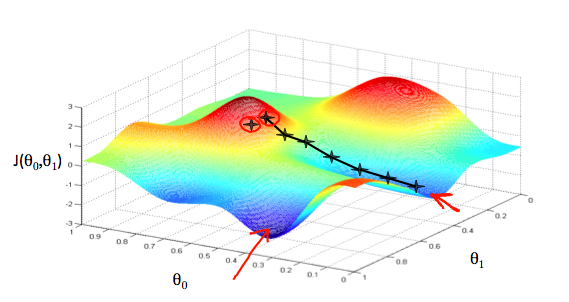
\includegraphics[width=1\textwidth]{img/bn9SyaDIEeav5QpTGIv-Pg_0d06dca3d225f3de8b5a4a7e92254153_Screenshot-2016-11-01-23.48.26.png}
    \caption{}\label{GradientDescent1}
\end{figure}
La figura \ref{GradientDescent1} mostra i punti risultati dal valore della funzione di costo nei punti $\Theta_0$ e $\Theta_1$. Le frecce rosse indicano alcuni dei possibili punti di minimo sul grafo. Il modo per fare ciò è quello di usare la \textbf{derivata} (la linea tangente alla funzione) della nostra funzione di costo. La pendenza (\textit{slope}) della tangente è la derivata in un punti e ci indica la direzione su cui "muoverci". In termini spiccioli: \textit{Scendiamo per la funzione di costo nella direzione con la discesa più ripida}. La \textbf{lunghezza} di ogni passo è determinato da un parametro, che precedentemente abbiamo chiamato \textbf{learning rate} $\alpha$. \\ Nella figura \ref{GradientDescent1} ogni "star" rappresentata sul grafo indica uno step determinato dal parametro $\alpha$. 
\begin{definizione}
    Un valore di $\alpha$ più piccolo darà vita a un passo in discesa più piccolo. Viceversa per valori più grandi.
\end{definizione}
\begin{definizione}
Dato un determinato valore di $\Theta_0$ e $\Theta_1$ (vale anche per i valori arbitrari dati a priori), la direzione da intraprendere è determinata dalla derivata parziale di della funzione di costo:
\[ \frac{\partial}{\partial \theta_j} J(\theta_0, \theta_1)\]
\end{definizione})  
L'algoritmo per la \textbf{discesa del gradiente} è il seguente:
\begin{algorithm}[H]
\begin{algorithmic}
        \While{La funzione non converge}
    \For{j = 0 to j = 1}
    \State{$\theta_j := \theta_j - \alpha \frac{\partial}{\partial \theta_j} J(\theta_0, \theta_1)$}
    \EndFor
    \EndWhile
    \end{algorithmic}
\end{algorithm}
Dove j indica gli indici delle features. A ogni iterazione $j$ i parametri $\Theta_j$ vengono aggiornati \textbf{simultaneamente}.\\
Immaginiamo ora di avere, per semplicità, un solo parametro $\Theta_1 \in \mathbb{R}$ da gestire:
\[\theta_1:=\theta_1-\alpha \frac{d}{d\theta_1} J(\theta_1)\]
Analizziamo una situazione fondamentale: il valore della derivata $\frac{d}{d\theta_1} J(\theta_1)$. Qualora essa sia \textbf{positiva} allora $\Theta_1$ è destinato a \textbf{diminuire}, e viceversa (fig \ref{GradientDescent2}).
\begin{figure}[h!]
    \centering
    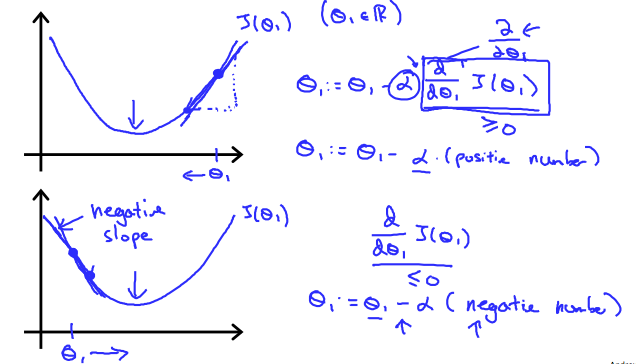
\includegraphics[width=1\textwidth]{img/SMSIxKGUEeav5QpTGIv-Pg_ad3404010579ac16068105cfdc8e950a_Screenshot-2016-11-03-00.05.06.png}
    \caption{}\label{GradientDescent2}
\end{figure}
\subsubsection{Descent Time}
A questo punto abbiamo intuito il perché molti denominano l'algoritmo come "\textit{Discesa del gradiente}", ma ci rimane da capire \textbf{quanto tempo} implica tale discesa.
In generale le tempistiche sono date da due fattori fondamentali:
\begin{itemize}
    \item Il valore di $\alpha$.
    \item Il valore della derivata.
\end{itemize}
Il primo aspetto da analizzare è la modifica del valore di $\alpha$ per garantire che il gradiente converga in un tempo accettabile. Un fallimento nella convergenza o una tempistica troppo elevata sono elementi caratterizzanti di un \textbf{learning rate} sbagliato.
\begin{figure}[h!]
    \centering
    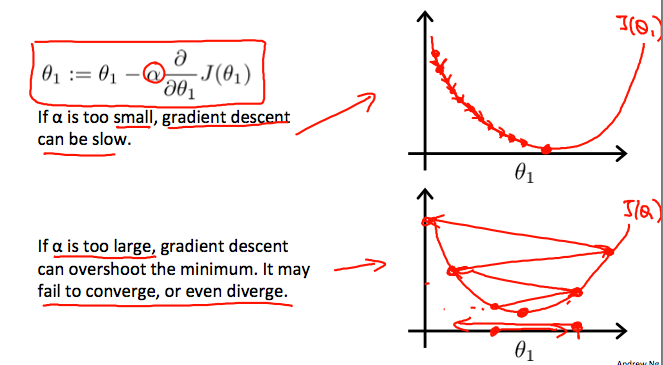
\includegraphics[width=1\textwidth]{img/UJpiD6GWEeai9RKvXdDYag_3c3ad6625a2a4ec8456f421a2f4daf2e_Screenshot-2016-11-03-00.05.27.png}
    \caption{}\label{GradientDescent3}
\end{figure}
Un'idea sarebbe quella di cambiare il valore di $\alpha$ al variare della discesa, in modo da evitare problematiche. Fortunatamente esiste un'intuizione che ci permette di far rimanere tale valore \textbf{costante} per tutto l'algoritmo. Ricordiamo infatti che il valore della derivata \textbf{diminuisce} a ogni passo. Questo poiché $\frac{d}{d\theta_1} J(\theta_1) \to 0$. Al minimo infatti avremo: 
\[\theta_1:=\theta_1-\alpha * 0\]
Quindi di step da effettuare diverranno sempre più piccoli.
\begin{figure}[h!]
    \centering
    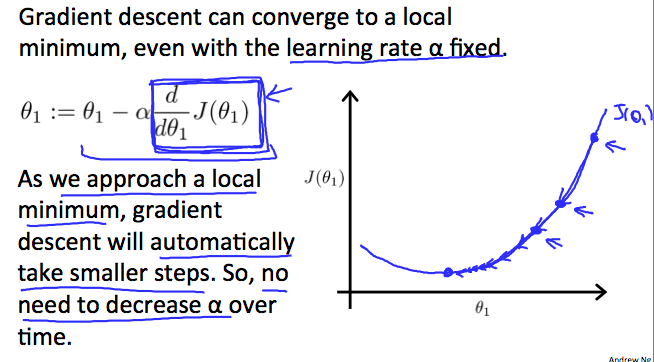
\includegraphics[width=1\textwidth]{img/RDcJ-KGXEeaVChLw2Vaaug_cb782d34d272321e88f202940c36afe9_Screenshot-2016-11-03-00.06.00.png}
    \caption{}\label{GradientDescent4}
\end{figure}
\subsubsection{Gradient Descent For Linear Regression}
Nelle reti neurali spesso si sfrutta quella che viene chiamata \textbf{Regressione lineare}, utilizzata soprattutto 
\section{Unità di calcolo nelle reti neurali}
Lo studio di un singolo neurone non è comunque particolarmente interessante. Si
introduce quindi lo studio di \textbf{reti neurali} dove vengono posti diversi
\textit{neuroni} in modo che possano fare qualcosa di utile.\\
Se dal singolo neurone voglio passare alla rete collego in modo orientato i
neuroni, di modo che l'output di uno sia l'input dell'altro. \\
Si hanno alcune \textbf{caratteristiche strutturali} delle \textit{reti neurali
artificiali}:
\begin{itemize}
	\item hanno un gran numero di unità
	\item permettono operazioni elementari
	\item hanno un alto livello d'interconnessione
\end{itemize}
Ci sono anche alcune \textbf{caratteristiche dinamiche}:
\begin{itemize}
	\item si hanno cambiamenti di stato in funzione dello stato dei neuroni
	      collegati in input
	\item si ha una funzione di uscita per ogni unità
	\item si ha la modifica dello schema di connessione, tramite la modifica dei
	      pesi, per l'apprendimento
\end{itemize}
Si hanno alcuni elementi caratterizzanti di una rete neurale:
\begin{itemize}
	\item il \textbf{tipo di unità}
	\item la \textbf{topologia}, ovvero la direzione delle connessioni
	      (\textit{feedforward \textnormal{o} feedback}), il numero di neuroni (con più
	      layer o solo uno, \textit{monostrato \textnormal{o} multistrato}) etc$\ldots$
	\item le \textbf{modalità di attivazione}, che può essere \textit{seriale
		ciclica, seriale probabilistica, parallela \textnormal{o} mista}
	\item un \textbf{algoritmo di apprendimento} con lo studio, in primis, dei
	      pesi
\end{itemize}
\newpage

Quindi le reti neurali sono composte da nodi o \textbf{unità} unite da \textbf{collegamenti} diretti. Un collegamento dall'unità $j$ all'unità $i$ serve a propagare l'attivazione $a_j$ da $j$ a $i$. A ogni collegamento è associato il \textbf{peso} $W_{j,i}$ che determina quindi la forza e il segno della connessione. La figura \ref{Neurone} ne mostra un esempio. 
\begin{figure}[h!]
	\centering
	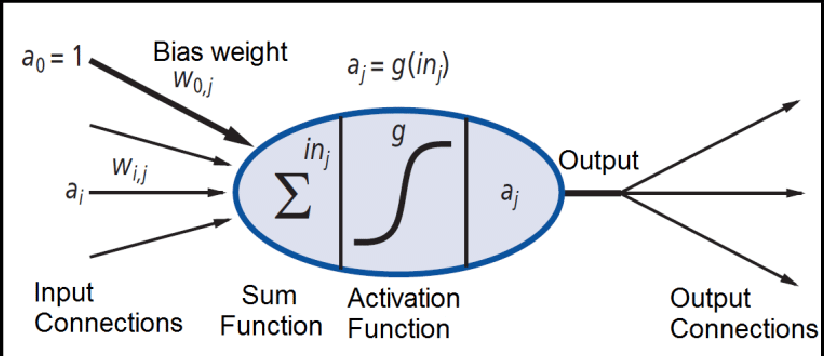
\includegraphics[width=0.75\textwidth]{img/An-artificial-neuron-and-its-various-components-Adapted-from-Norvig-Russel-2013-p.png}
	\caption{Neurone Artificiale}
	\label{Neurone}
\end{figure}
Ogni unità $i$ calcola per prima cosa una somma pesata dei propri input:
\[in_i=\sum_{j=0}^n W_{j,i}\cdot a_j\]
Fatto questo, applica una \textbf{funzione di attivazione} $g$ alla somma per derivare l'output:
\[a_i=g(in_i)=g\left(\sum_{j=0}^n W_{j,i}\cdot a_j\right)\]
La funzione di attivazione $g$ può essere strutturata in diversi modo ed è progettata per soddisfare due requisiti:
\begin{itemize}
	\item Prima di tutto desideriamo che l'unità sia attiva (vicina ad 1) quando sono dati i valori giusti di input, altrimenti vogliamo che essa sia inattiva (vicina a -1).
	\item L'attivazione deve essere non lineare.
\end{itemize}
\textbf{NOTA:} L'output di un neurone (quindi il risultato della funzione di attivazione) è, a conti fatti, uno stato ($a_i$) per un altro neurone. Quindi esiste una relazione tra $a_i$ e $g$.\\
La funzione di attivazione $g$ può essere rappresentata da diverse funzioni, tra cui:
\begin{itemize}
	\item La funzione Soglia
	\item La funzione Sigmoide/Logistica
\end{itemize}
\begin{figure}[h!]
	\centering
	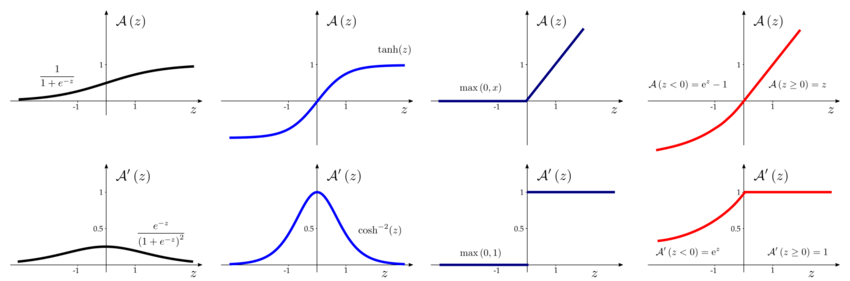
\includegraphics[width=1\textwidth]{img/Some-of-the-most-common-activation-functions-and-their-first-order-gradient-From-left-to.png}
	\caption{Funzioni di Attivazione}
	\label{ActivationFunction}
\end{figure}
L'insieme degli stati, rappresentato in modo binario, comporta che la funzione
di transizione sia una \textbf{funzione soglia}:
\[g(in_i)=
	\begin{cases}
		1 & \mbox{se } in_i\geq \theta \\
		0 & \mbox{altrimenti}                                   
	\end{cases}\,\,\,\mbox{con $in_i = \sum_{j=0}^n W_{j,i}\cdot a_j$}
\]
Questo modello è comunque estremamente semplificato. L'insieme degli stati potrebbe non essere booleano ma potrebbe essere $\mathbb{R}$, infatti anche nella biologia il segnale in uscita dai neuroni è graduato e continuo. \\
Si potrebbe quindi avere una \textbf{funzione logistica o sigmoide}, dove, avendo come insieme degli stati $\mathbb{R}$ si avrebbe:
\[f(x)=\frac{1}{1+e^{-x}}\]
I lettori a questo punto si porranno la seguente domanda: "Mario, allora come possiamo capire quando la funzione $g$ soddisfa un determinato input $in_i = W_{j,i}\cdot a_j$ all'interno di un'unità?". Solitamente si fa riferimento al peso di \textbf{bias} indicato da $W_{0,j}$ che determina la soglia effettiva dell'unità, sebbene spesso essa sia uguale a zero. In particolare esiste anche un \textbf{nodo di bias}  che possiede un determinato stato (indicato solitamente con $a_0$ o, nel caso in cui sia un nodo in input alla rete, $x_0$) normalmente posto uguale ad $1$ (sopratutto nel neurone binario).\\
\textbf{NOTA:} L'uscita della rete può essere simboleggiato in diversi modi, solitamente i diversi testi si accordano su una delle seguenti nomenclature: $y, h_\theta(x), h_W(x)$. Quindi non bisogna confondersi qualora in un esempio comparisse $h_\theta(x)$ al posto di $h_W(x)$.\\
\textbf{NOTA:} Per definire i \textbf{due stati del neurone binario} si usa l'insieme $\{0, 1\}$ o l'insieme $\{-1, 1\}$.
\section{Struttura della rete}
Ci sono due categorie principali di strutture di reti neurali:
\begin{itemize}
	\item Feed-Forward / Alimentata in avanti
	\item Ricorrenti
\end{itemize}
Questo libro si concentrerà sulle strutture \textbf{Feed-Forward}. Esse sono abitualmente organizzare in \textbf{strati}, in modo tale che ogni unità riceva in input solo dalle unità nello strato immediatamente precedente. Oltretutto esse permettono anche la possibilità di avere degli strati nascosti e, di conseguenza, delle unità nascoste. In questa sezione introdurremo due tipologie di reti neurali:
\begin{itemize}
	\item Single Layer: 
	      Nelle reti neurali a \textbf{single layer} un insieme d'input è direttamente mappato su un layer di output. Questa semplice istanziazione di rete è anche chiamata come \textit{percettrone}.
	\item Multi Layer: dove il layer d'input e quello di output sono separati da un gruppo di \textbf{layer nascosti}. 
\end{itemize}
\textbf{NOTA:} Solitamente nell'\textbf{input layer} i nodi in input vengono descritti da un \textbf{vettore} $X$.
\subsection{Reti neurali a uno strato alimentate in avanti: il percettrone}
Questa tipologia di architettura possiede un singolo \textbf{input layer} e un \textbf{output layer}. La figura \ref{Percettrone} mostra un esempio della struttura.
\begin{figure}[h]
	\centering
	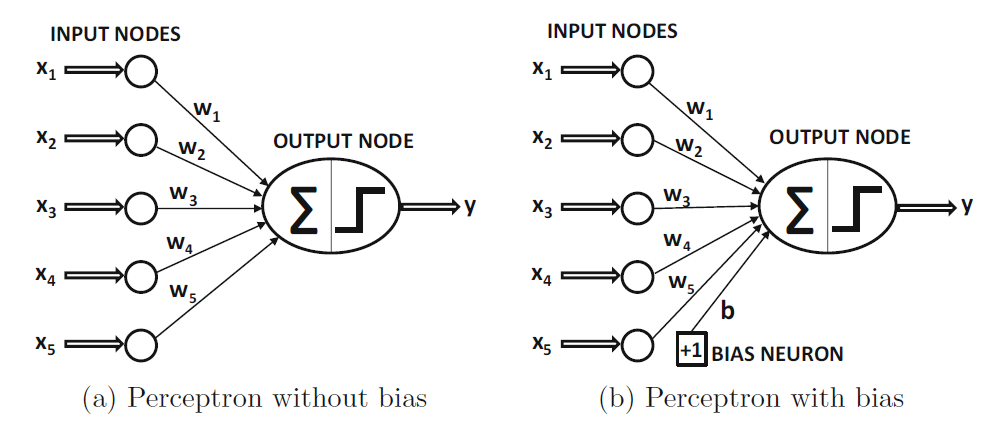
\includegraphics[width=1\textwidth]{img/Capture.PNG}
	\caption{Percettrone}
	\label{Percettrone}
\end{figure}
\begin{definizione}
	Un percettrone è una collezione di neuroni, di cardinalità $M$, a cui viene
	aggiunto un insieme di nodi in input, di cardinalità $N$ (generalmente
	diversa da quella della collezione di neuroni). Generalmente gli input sono
	pesati e con la notazione $w_{ij}$ indichiamo il peso della connessione tra il
	nodo $i$-simo in input e il neurone $j$-simo.\\
	I neuroni sono tra loro completamente indipendenti comportando anche un
	insieme di elementi in output. Nel caso semplice di funzioni di transizione
	binarie l'output sarà quindi un vettore binario contenente all'indice $k$-simo
	1 se il neurone $k$ ha inviato il segnale o 0 altrimenti. \\
	Solitamente coi percettroni si parla di \textit{learning supervisionato}.
\end{definizione}
Sappiamo che un percettrone a \textbf{soglia} restituisce 1 se e solo se la somma pesata dei suoi input (bias incluso) è positiva:
\[\sum_{j=0}^n W_j\cdot x_j > 0\]\,\,\,\mbox{oppure}\,\,\,\[W\cdot x > 0\]
Dal punto di vista geometrico l'equazione $W\cdot x$ rappresenta un 
\textbf{iperpiano} nello spazio d'input (che è una retta in $\mathbb{R}^2$) che separa i possibili
vettori d'input in due classi, a seconda che formino con $W$ un angolo acuto o
ottuso. Quindi il percettrone restituisce $1$ se e solo se l'input si trova da una parte specifica rispetto a tale iperpiano. Per questa ragione, il percettrone a soglia è chiamato anche \textbf{separatore lineare}. Difatti esso può rappresentare \textbf{funzioni linearmente separabili} (fig. \ref{SeparatoreLineare}).\\
\begin{figure}[h!]
	\centering
	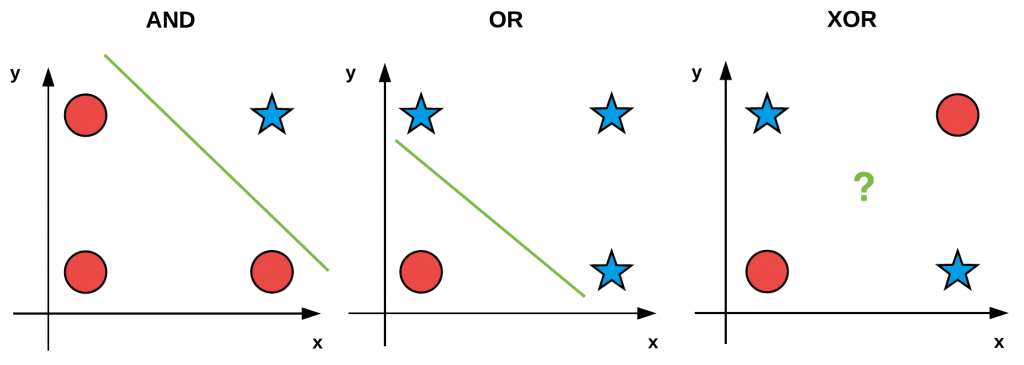
\includegraphics[width=1\textwidth]{bitwise_datasets-1024x365.png}
	\caption{Separatore Lineare}
	\label{SeparatoreLineare}
\end{figure}
È chiaro quindi che i \textbf{percettroni a soglia possono rappresentare solo funzioni linearmente separabili}. D'altro Canto esiste un semplice algoritmo di apprendimento capace di adattare un percettrone a soglia a qualsiasi insieme di addestramento linearmente separabile.
\subsubsection{Algoritmo del percettrone e Discesa del Gradiente}
Fino a ora il singolo neurone rappresentava un singolo iperpiano che veniva ``spostato'' per dividere le istanze positive e quelle negative. Ora introduciamo che a ogni passo di aggiornamento si aggiornano i pesi e se, mano a mano che cambio i pesi, misuro l'errore sul dataset del mio sistema. Si può quindi far ``scendere'' questo errore e ci si augura che ci sia una costante di discesa dell'errore. L'idea di questo algoritmo è di calibrare i pesi nella rete in modo da minimizzare una qualche misura di errore sull'insieme di training. Quindi L'apprendimento è formulato come una ricerca di ottimizzazione nello \textbf{spazio dei pesi}. La misura di errore è la \textbf{somma dei quadrati degli errori}.
Il quadrato dell'errore per un singolo esempio di training con input $x$ e output $y$ si scrive:
\[E=\frac{1}{2}(y-h_W(x))^2\]\mbox{Dove $h_W(x)$ è l'output del percettrone per l'esempio.}
Se indicassimo $Err = (y-h_W(x))$ allora la formula si potrebbe trascrivere come:
\[E=\frac{1}{2}(Err)^2\]\mbox{Dove $h_W(x)$ è l'output del percettrone per l'esempio.}

Possiamo usare il \textbf{metodo della discesa di gradiente} per ridurre il quadrato dell'errore calcolando la derivata parziale di $E$ rispetto a ogni peso: 
\[\frac{\partial E}{\partial W_j} = - Err \times g'(in) \times x_j\] 
Nell'algoritmo a discesa del gradiente, in cui vogliamo \textbf{ridurre} E, aggiorniamo i pesi come segue:
\[W_{j}\gets W_{j}+\alpha\cdot Err \times g'(in) \times x_j\]
Nel caso in cui si trattasse percettroni con funzione di attivazione a soglia, allora la formula diventa:
\[W_{j}\gets W_{j}+\alpha\cdot Err \times x_j\]
Si calcola il gradiente della curva degli errori e si punta a essere sempre in ``discesa'' lungo la curva dell'errore, aggiustando in modo opportuno i pesi. Viene anche introdotto il \textbf{learning rate (\textit{tasso di apprendimento})} $\alpha$, utile per stabilire la velocità di apprendimento della rete. In pratica $\alpha$ decide quanto cambiare il peso (e se si vuole trascurare il parametro basta porre $\alpha =1$). L'uso di tale parametro migliora la stabilità della \textit{rete neurale} che non avrà cambi di peso eccessivi, anche se
questo comporta tempi di apprendimento più estesi. Tipicamente si ha che:
\[0.1\leq\alpha\leq 0.4\]
Si noti che se l'errore $y-h_W(x)$ è positivo allora $y>h_W(x)$ quindi l'output della rete dev'essere troppo piccolo e quindi i pesi aumentano per gli input positivi e diminuiscono per quelli negativi. Quando l'errore è negativo avviene l'opposto. La procedura si potrebbe iterare \textbf{ipoteticamente} finché non si arriva ad avere un output \textit{"uguale"} a quello del dataset. Gli esempi di addestramento vengono fatti passare attraverso la rete uno per volta, modificando leggermente i pesi a ogni iterazione per ridurre l'errore. Ogni ciclo attraverso tutti gli esempi prende il nome di \textbf{epoca}. Le epoche sono tipicamente ripetute fino a quando non viene soddisfatto qualche criterio di terminazione. Si ha che a ogni iterazione ci si aspetta un miglioramento della \textit{rete neurale} (e questo miglioramento è dimostrabile). Viene imposto
quindi un limite $T$ d'iterazioni entro le quali interrompere l'apprendimento anche se non si è arrivati al risultato
corretto.

Vediamo quindi l'algoritmo di apprendimento del percettrone:
\begin{algorithm}[H]
	\begin{algorithmic}
		\Function{perceptron-learning}{esempi, rete}
		\State{\textbf{inputs:} esempi, un insime di esempi, ognuno con input $x=x\dots x_n$ e output $y$\\ rete, un percettrone con pesi $W_j=0\dots n$ e funzione di attivazione $g$}
		\For {\textit{$T$ iterazioni \textbf{o} fino a che tutti gli output non sono
		corretti}}
		\For {\textbf{each} $e$ in \textit{esempi}}
		\State{$in \gets \sum_{j=0}^n W_j\cdot x_j[e]$}
		\State{$Err \gets y[e] - g(in)$}
		\State $W_{j}\gets W_{j}+\alpha\cdot Err \times g'(in)\times x_j[e]$
		\EndFor
		\EndFor
		\EndFunction
	\end{algorithmic}
	\caption{Algoritmo di learning del percettrone}
\end{algorithm}
La complessità dell'algoritmo è $O(Tnm)$.\\
% \begin{algorithm}[h] % TODO: modify
% 	\begin{algorithmic}
% 		\Function{grad}{}
% 		\State \textit{inizializzo ogni $\Delta w_i$ a $0$}
% 		\For {\textit{ogni input $\langle( x_1, \ldots x_n), t\rangle$}}
% 		\State \textit{invio l'input $( x_1, \ldots x_n)$ all'unità lineare e
% 		calcola l'output $y$} 
% 		\State \textit{aggiorno la variazione dei pesi:}
% 		\[\Delta w_i=\Delta w_i+\alpha\cdot (t-y)\cdot x_i\]
% 		\EndFor
% 		\State \textit{aggiorno i pesi:}
% 		\[w_i=w_i+\Delta w_i\]
% 		\EndFunction
% 	\end{algorithmic}
% 	\caption{Algoritmo di discesa lungo il gradiente}
% \end{algorithm}
% Abbiamo una \textbf{modalità Batch}, quindi computazionalmente costosa:
% \[w=w-\alpha\cdot\nabla E_D[W]\]
% Si può avere una \textbf{modalità incrementale}:
% \[w=w-\alpha\cdot\nabla E_d[W]\]
% calcolata sui singoli esempi $d$:
% \[E_d[w]=\frac{1}{2}(t_d-y_d)^2\]
% La discesa lungo il gradiente incrementale può approssimare la discesa lungo
% il gradiente Batch arbitrariamente se $\alpha$ è abbastanza piccolo.\\
% Rispetto a quanto visto per il percettrone la discesa lungo il gradiente
% converge all'ipotesi con il minimo errore quadratico se  $\alpha$ è abbastanza
% basso, anche per dati di training molto rumorosi.

% \[\Delta w_{ik}=-(y_k-t_k)\times a_i\]
% In questo discorso bisogna inserire anche la soglia, importante per input
% specifici (basti pensare a un input pari a 0 che annullerebbe ogni cambio di
% peso secondo la formula precedente). Per ora trascureremo tali casi anche se una
% semplice soluzione per un caso limite come quello di avere solo input nulli, è
% quella di aggiungere un \textbf{nodo bias}, di valore $-1$, collegato ai neuroni
% con peso nullo.\\


\subsubsection{Approfondimento sul Percettrone}
Vediamo due teoremi utili per lo studio dell'apprendimento del percettrone su due classi $A$ e $B$, banalmente rappresentanti, nella nostra situazione binaria e semplificata, il caso in cui si abbia il neurone che emette il segnale (valore 1 in output) o altrimenti (valore 0 in output). Nel nostro caso le classi sono discriminabili.
\begin{definizione}[definizione di convergenza]
	Comunque si scelgano i pesi iniziali, se le classi A e B sono discriminabili,
	la procedura di apprendimento termina dopo un numero finito di passi
\end{definizione}
\begin{definizione}[definizione di Minsky e Papert]
	La classe delle forme discriminabili da un percettrone semplice è
	limitata alle forme linearmente separabili
\end{definizione}
In base a questo si distinguerà in:
\begin{itemize}
	\item \textbf{addestramento separabile}, quando si ha un iperpiano che separa
	      le istanze positive e negative
	\item \textbf{addestramento non separabile}
\end{itemize}
Per capire il discorso della \textbf{separabilità} vediamo un esempio.
\begin{esempio}
	Vediamo un esempio che tratta l'addizione binaria, ovvero l'\textit{or
	esclusivo}.
	Le possibili istanze sono rappresentate nel piano:
	\begin{figure}[H]
		\centering
		\psscalebox{1.0 1.0} % Change this value to rescale the drawing.
		{
			\begin{pspicture}(0,-1.9534792)(5.906958, 1.9534792)
				\psline[linecolor=black, linewidth=0.04,
					arrowsize=0.05291667cm 2.0, arrowlength=1.4
				, arrowinset=0.0]{->}(2.4,-1.9534792)(2.4, 1.6465209)(2.4, 2.046521)
				\psline[linecolor=black, linewidth=0.04,
					arrowsize=0.05291667cm 2.0, arrowlength=1.4,
				arrowinset=0.0]{->}(1.6,-1.1534791)(6.0,-1.1534791)
				\psdots[linecolor=black, dotsize=0.4](2.4, 0.84652084)
				\psdots[linecolor=black, dotsize=0.4](4.4, 0.84652084)
				\psdots[linecolor=black, dotsize=0.4](4.4,-1.1534791)
				\psdots[linecolor=black, dotsize=0.4](2.4,-1.1534791)
				\rput[bl](0.4, 0.68652084){$0\oplus 1=1$}
				\rput[bl](0.4,-0.7534792){$0\oplus  1=0$}
				\rput[bl](3.4,-0.7534792){$1\oplus 0=1$}
				\rput[bl](3.4, 1.2465209){$1\oplus 1=0$}
			\end{pspicture}
		}
	\end{figure}
	Ho quindi che nessuna retta potrà separare tutti i punti e
	quindi i punti a valore 1 \textbf{non sono linearmente separabili} da quelli a
	valore 0.\\
	Si vorrebbe cercare un neurone binario a soglia tale che:
	\[x\oplus y=1\iff \alpha\cdot x+\beta\cdot y\geq \alpha\]
	Tale neurone si rappresenterebbe con:
	\begin{figure}[H] 
		\centering
		\psscalebox{1.0 1.0} % Change this value to rescale the drawing.
		{
			\begin{pspicture}(0,-1.9534792)(5.906958, 1.9534792)
				\pscircle[linecolor=black, linewidth=0.04,
				dimen=outer](3.2, 0.24245118){0.8}
				\psline[linecolor=black, linewidth=0.04,
					arrowsize=0.05291667cm 2.0, arrowlength=1.4,
				arrowinset=0.0]{->}(0.4, 0.64245117)(2.4, 0.64245117)
				\psline[linecolor=black, linewidth=0.04, arrowsize=0.05291667cm 2.0,
				arrowlength=1.4, arrowinset=0.0]{->}(0.4,-0.15754883)(2.4,-0.15754883)
				\psline[linecolor=black, linewidth=0.04, arrowsize=0.05291667cm 2.0,
				arrowlength=1.4, arrowinset=0.0]{->}(4.0, 0.24245118)(6.0, 0.24245118)
				\rput[bl](0.0, 0.56245117){$x$}
				\rput[bl](0.0,-0.32754883){$y$}
				\rput[bl](1.2, 0.8245117){$\alpha$}
				\rput[bl](1.2, 0.024245118){$\beta$}
				\rput[bl](3.07, 0.115754886){$\alpha$}
				\rput[bl](6.2, 0.0824245118){$x\oplus y$}
			\end{pspicture}
		}
	\end{figure}
	ma appunto tale neurone non può esistere in quanto non potrei mai separare
	i punti a valori 1 e quelli a valore 0 con una retta. Posso infatti separare o
	singoli punti o coppie di punti a valore opposto o triple di punti ma non
	potrò mai avere separati insiemi con tutti gli 0 e tutti gli 1.
\end{esempio}
\begin{definizione}
	Se l'insieme degli input estesi è partito in due classi linearmente separabili
	allora:
	\[\exists\,\, W\mbox{t.c }
		\begin{cases}
			1 & \mbox{se } \sum w_i\cdot a_i \geq 0 \\
			0 & \mbox{se } \sum w_i\cdot a_i < 0    
		\end{cases}
	\]
	con $W$ \textbf{vettore dei pesi}.
\end{definizione}
Vediamo quindi l'algoritmo di learning per un percettrone, data la
\textbf{funzione di attivazione} per un input di cardinalità $m$ e $n$ neuroni:
\[
	y_j=g\left(\sum_{i=0}^m w_{ij}\cdot a_i \right)=
	\begin{cases}
		1 & \mbox{se } \sum_{i=0}^m w_{ij}\cdot a_i > 0    \\
		0 & \mbox{se } \sum_{i=0}^m w_{ij}\cdot a_i \leq 0 
	\end{cases}
\]
Si può dimostrare, tramite il \textbf{definizione della convergenza del percettrone}
che dopo $\beta$ modifiche di peso il percettrone classifica 
correttamente ogni input anche se tale $\beta$ non è il reale numero di stadi e
dipende dall'output.\\
L'algoritmo di apprendimento del percettrone quindi \textit{converge} alla
classificazione corretta quindi se:
\begin{itemize}
	\item i dati di training sono linearmente separabili
	\item $\alpha$ è abbastanza piccolo
\end{itemize}
% \begin{definizione}
% 	Se l'insieme degli input estesi è partito in due classi linearmente separabili
% 	$A$ e $B$ allora é possibile trovare un vettore di pesi $w$ tale che:
% 	\[
% 		\begin{cases}
% 			\langle w, x\rangle\geq 0 & \mbox{se }x\in A \\
% 			\langle w, x\rangle < 0   & \mbox{se }x\in B 
% 		\end{cases}
% 	\]
% 	Quindi:
% 	\begin{itemize}
% 		\item si parte con $w$ arbitrario
% 		\item si classifica un punto $x$:
% 		      \begin{itemize}
% 		      	\item se la risposta è corretta si ha $w'\gets w$
% 		      	\item se la risposta è errata:
% 		      	      \[
% 		      	      	\begin{cases}
% 		      	      		w'\gets w+x & \mbox{se }x\in A \\
% 		      	      		w'\gets w-x & \mbox{se }x\in B \\
% 		      	      	\end{cases}
% 		      	      \]
% 		      \end{itemize}
% 	\end{itemize}
	
% \end{definizione}
% \begin{proof}
% 	Vediamo la prova della correttezza del definizione.\\
% 	Se si ha $x\in A$ allora si ha $\langle w, x\rangle<0$ infatti, poiché:
% 	\[\langle x, x\rangle\geq 0\]
% 	si ha che:
% 	\[\langle w', x\rangle=\langle (w+x), x\rangle=\langle w, x\rangle+\langle x,
% 		x\rangle>\langle w, x\rangle\]
% 		Quindi $w'$ classifica $x$ in modo più corretto di $w$ anche se altri input
% 		possono essere classificati "meno correttamente".
% 		\end{proof}
% 		\begin{proof}
% 			Passiamo ora alla convergenza.\\
% 			Consideriamo quindi $A'=A\cup B'$ con:
% 			\[B'=\{-x|\, x\in B\}\]
% 			e cerchiamo un $v$ tale che:
% 			\[\langle v, x\rangle\geq 0,\,\,\forall\, x\in A'\]
% 			Si hanno quindi:
% 			\begin{itemize}
% 				\item la \textbf{sequenza di addestramento} $\{x_i\}_{i\in N}$ dove $x_i\in
% 				      A'$ e quindi la sequenza ontiene infiniti elementi sia di $A$ che di $B'$
% 				\item la \textbf{sequenza di pesi} $\{w_i\}_{i\in N}$ dove si parte
% 				      arbitrariamente con $w_0=0$ e si procede con:
% 				      \[
% 				      	\begin{cases}
% 				      		w_{k+1}\gets w_k     & \mbox{se }\langle w_k, x_k\rangle\geq 0 \\
% 				      		w_{k+1}\gets w_k+x_k & \mbox{altrimenti}                       
% 				      	\end{cases}
% 				      \]
% 			\end{itemize}
% 			Si hanno quindi:
% 			\begin{itemize}
% 				\item la \textbf{sequenza di pesi modificata} $\{v_i\}_{i\in N}$ 
% 				\item la \textbf{sottosequenza di training corrispondente} $\{v_i\}_{i\in N}$ 
% 			\end{itemize}
% 			Di modo che le coppie $(v_i, t_i)$ corrispondano ai $w_j$ tali per cui $w_j\neq
% 			w_{j+1}$.\\
% 			Ad esempio per:
% 			\[w_0\neq w_1=w_2=w_3\neq w_4=w_5=w_6\neq w_7\neq w_8\cdots\]
% 			avremo:
% 			\begin{itemize}
% 				\item $(v_0, t_0)$ associati a $w_0$
% 				\item $(v_1, t_1)$ associati a $w_3$
% 				\item $(v_2, t_2)$ associati a $w_6$
% 				\item $(v_3, t_3)$ associati a $w_7$
% 			\end{itemize}
% 			Avendo:
% 			\[\langle v_i, t_i\rangle<0\,\,\,\forall i\]
% 			e avendo:
% 			\[v_{i+1}=v_i+t_i=v_{i-1}+t_{i-1}+y_i=\sum_{k=0}^i t_i\]
% 			e quindi la sequenza $\{v_i\}$ è \textbf{finita}.
% 		\end{proof}
% 		\begin{proof}
% 			Uniamo matematicamente in una sola dimostrazione.\\
% 			Sia $w$ una qualsiasi soluzioni che sappiamo esistere per ipotesi. Si ha che:
% 			\[\langle v, x\rangle\geq 0,\,\,\forall\, x\in A'\]
% 			Pongo quindi:
% 			\[\alpha=\min(\langle x, w\rangle,\,\,\forall\, x\in A')\]
% 			sapendo che:
% 			\[v_{i+1}=v_i+t_i=v_{i-1}+t_{i-1}+y_i=\sum_{k=0}^it_i\]
% 			ho che:
% 			\[\langle v_{i+1}, w\rangle=\langle \left(\sum_{k=0}^i t_k \right),
% 				w\rangle\geq (i+1)\cdot\alpha\]
% 				ma usando il definizione di \textbf{Cauchy-Schwarz} si ha che:
% 				\[(\langle v_{i+1}, w\rangle)^2\leq \langle |v_{i+1}|^2,|w|^2\rangle\]
% 				ottenendo che:
% 				\[|v_{i+1}|^2\geq \frac{(i+1)^2\cdot \alpha^2}{|w|^2}\]
% 				Pongo quindi:
% 				\[M=\max\{|x|^2|,\, x\in A'\}\]
% 				si ha che, avendo $\langle v_{1}, t_i\rangle<0$:
% 				\[|v_{i+1}|^2=|v_i+t_i|^2=|v_i|^2+2\cdot\langle v_{i}, t_i\rangle+|t_i|^2\leq
% 					|v_i|^2+|t_i|^2\]
% 					Si ha, di conseguenza:
% 					\[|v_{i+1}|^2\leq \sum_{k=1}^i |t_i|^2\leq i\cdot M\]
% 					Unendo quest'ultima con $|v_{i+1}|^2\geq \frac{(i+1)^2\cdot \alpha^2}{|w|^2}$
% 					si ha che:
% 					\[f(i)=\frac{j^2\cdot \alpha^2}{|w|^2}\leq |v_{i+1}|^2\leq i\cdot M=g(i)\]
% 					avendo che $\frac{j^2\cdot \alpha^2}{|w|^2}$ è quadratico in $i$ e $ i\cdot M$
% 					lineare in $i$.\\
% 					Si ottiene quindi che:
% 					\[i\leq\frac{M\cdot |w|^2}{\alpha^2}=\beta\]
% 					Quindi dopo $\beta$ modifiche di peso il percettrone classifica correttamente
% 					ogni input.
% 					\end{proof}
					\subsubsection{Adeline vs Percettrone}
					Il percettrone si basa su un'unica unità di calcolo e tramite una funzione
					soglia valorizza l'uscita in modo da farle assumere un valore booleano in
					$\{-1, 1\}$.\\
					Si hanno vari pesi $w_i$ che scalano l'ingresso e, insieme agli input $x_i$
					(compreso l'input bias),
					formano il \textbf{potenziale di attivazione}:
					\[\sum_{i=0}^nw_ix_i=\langle \overline{w}, \overline{x}\rangle\]
					che verrà poi fatto passare per la funzione
					soglia. Se il potenziale è positivo si avrà uno in uscita, se negativo o nullo
					-1:
					\[output=
						\begin{cases}
							1  & \mbox{se } \sum w_i\cdot x_i > 0    \\
							-1 & \mbox{se } \sum w_i\cdot x_i \leq 0 
						\end{cases}
					\]
					In letteratura si hanno modelli dove il potenziale nullo comporta una terza
					uscita pari a 0.\\
					Il percettrone basa il suo algoritmo di training su un ciclo che aggiorna di
					volta in volta i pesi intermedi.
					Per il percettrone si ha quindi una funzione di aggregazione del tipo:
					\[z=b+\sum_{i=1}^nw_ix_i\]
					(con $b$ valore del nodo bias)\\
					che viene passata alla funzione soglia:
					\[f(z)=\hat{y}\]
					calcolando l'output:
					\[\hat{y}\in\{-1, 1\}\]
					Per aggiornare i pesi si calcola l'errore (la differenza tra il valore calcolato
					$\hat{y}$ e la label associata all'esempio in analisi $y$):
					\[error=y-\hat{y}\]
					calcola la correzione del peso, tramite la fattorizzazione dei pesi:
					\[\Delta w=\alpha(error)x_k\]
					e aggiornando poi i pesi:
					\[w_{k+1}=w_k+\Delta w_k\]
					Nel caso di Adaline si ha una struttura in realtà simile ma utilizza una
					valutazione nel continuo degli errori, ad esempio tramite una certa funzione
					lineare. La funzione prende prende in input il potenziale di attivazione e la
					cui uscita viene valutata per il calcolo dell'errore $\delta$ tramite la
					\textbf{$\delta$ rule} ($\delta$ che ha valore continuo e non booleano). Si ha
					comunque una funzione di uscita a soglia che funziona come per il percettrone
					standard, se positivo il risultato restituisce 1 altrimenti -1.\\
					Per Adaline si ha quindi una funzione di aggregazione del tipo:
					\[\hat{y}=b+\sum_{i=1}^nw_ix_i\]
					(con $b$ valore del nodo bias)\\
					che viene passata alla funzione soglia:
					\[f(\hat{y})\]
					per produrre l'uscita booleana (uguale al percettrone):
					\[\hat{y}'\in\{-1, 1\}\]
					per l'update dell'errore, a partire dalla funzione di aggregazione, si procede
					circa come per il percettrone standard, avendo però un errore quadratico:
					\[error=(y-\hat{y})^2\]
					e avendo poi l'update tramite:
					\[w_{k+1}=w_k-\alpha(2error_k)x_k\]
					Riassumendo abbiamo l'algoritmo del percettrone che, per ogni esempio $\langle
					x, t\rangle$ con $t$ label, esegue:
					\begin{enumerate}
						\item $y=step(f(x))$ (con step che da il booleano a seconda del segno)
						\item $w=w+\alpha(t-y)x$
					\end{enumerate}
					Si ha che:
					\begin{itemize}
						\item se l'output matcha il target allora $t-y$ è nullo e non si aggiornano i
						      pesi
						\item se l'output è 1 ma il target è 0 l'input, scalato con learning rate
						      $\alpha$, viene sottratto dal vettore dei pesi
						\item se l'output è 0 ma il target è 1 l'input, scalato con learning rate
						      $\alpha$, viene aggiunto al vettore dei pesi
					\end{itemize}
					Riassumendo abbiamo l'algoritmo del Adaline che, per ogni esempio $\langle
					x, t\rangle$ con $t$ label, esegue:
					\begin{enumerate}
						\item $y=f(x)$
						\item $w=w+\alpha(t-y)x$
					\end{enumerate}
					Si ha che questo equivale la regola del \textit{gradient descent} della
					regressione lineare (con errore quadratico), infatti la derivata di $(y-t)^2$ è
					$2(z-t)$. Il fattore costante 2 può essere omesso dato che si usa il learning
					rate per rimodulare quanto aggiornare i pesi.\\
					Ovviamente entrambi possono studiare solo set di punti separabili linearmente,
					usando iperpiani e non rette se saliamo di grado su $\mathbb{R}$, per separare i
					punti.
					\subsubsection{Esercizi guidati}
					\begin{esercizio}
						Prendiamo il seguente training set con $t(x)$ che ci fornisce la label:
						\begin{table}[H]
							\centering
							\begin{tabular}{c||c|c|c}
								      & $x$ & $y$  & $t(x)$ \\
								\hline
								\hline
								$x_1$ & 1   & 1    & 1      \\
								$x_2$ & 2   & -2   & -1     \\
								$x_3$ & -1  & -1.5 & 1      \\
								$x_4$ & 1   & -2   & -1     \\
								$x_5$ & -2  & -1   & 1      \\
							\end{tabular}
						\end{table}
						graficamente possiamo rappresentare tali punti (in blu con target $+1$ e rosso
						per target $-1$, notando che sono linearmente separabili):
						\begin{figure}[H]
							\centering
							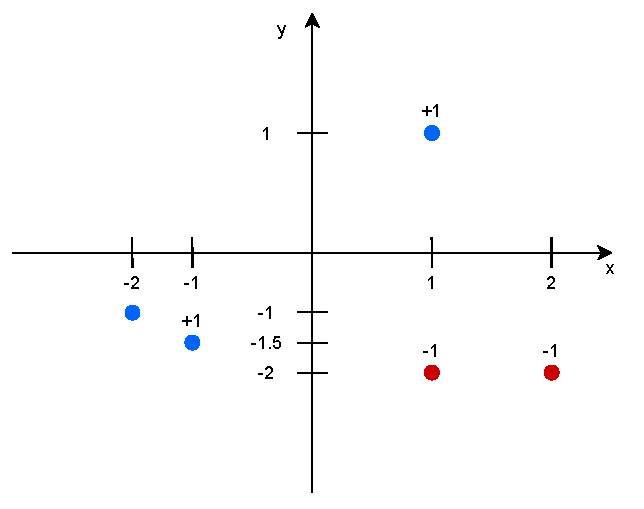
\includegraphics[scale = 0.8]{img/per1.pdf}
						\end{figure}
						Usiamo quindi l'algoritmo del percettrone e studiamo come si aggiornano i
						pesi. Si impone $\alpha=0.2$ e nodo bias di valore $b=1$ e peso $w_0$,
						arbitrariamente inizializzato a 0.\\ 
						Partiamo con il primo esempio. Si hanno:
						\begin{itemize}
							\item $x_1=(1, 1)$
							\item $t(x_1)=1$
						\end{itemize}
						da ciò si ricava che l'input del percettrone, il suo segnale d'ingresso, altro
						non è che, considerando il nodo bias:
						\[\overline{x}=(b, x_1)=(1, 1, 1)\]
						Arbitrariamente inizializziamo i pesi a (avendo già detto che il bias ha peso
						0):
						\[\overline{w}=(0, 1, 0.5)\]
						Faccio quindi il prodotto scalare tra il vettore input e il vettore peso:
						\[\langle \overline{w}, \overline{x}\rangle=
							\left(\begin{matrix}
							0 & 1 & 0.5
							\end{matrix}\right)
							\left(
							\begin{matrix}
								1 \\
								1 \\
								1 \\
							\end{matrix}
							\right)= 0 + 1 + 0.5 = 1.5
						\]
						Si ha quindi $\langle \overline{w}, \overline{x}\rangle > 0$ e quindi:
						\[g(\langle \overline{w}, \overline{x}\rangle)=+1\]
						e avendo che, ricordando $t(x_1)=+1$:
						\[g(\langle \overline{w}, \overline{x}\rangle)=t(x_1)\]
						i pesi $\overline{w}$ non devono essere aggiornati.\\
						Si passa al secondo esempio.\\
						Si ha (senza dover rispiegare gli step metto tutto nella stessa lista):
						\begin{itemize}
							\item $x_2=(2,-2)$
							\item $t(x_2)=-1$
							\item $\overline{x}=(1, 2,-2)$
							\item $\overline{w}=(0, 1, 0.5)$
						\end{itemize}
						calcolo:
						\[\langle \overline{w}, \overline{x}\rangle=
							\left(\begin{matrix}
							0 & 1 & 0.5
							\end{matrix}\right)
							\left(
							\begin{matrix}
								1  \\
								2  \\
								-2 \\
							\end{matrix}
							\right)= 0 + 2 - 1 = 1
						\]
						Si ha quindi $\langle \overline{w}, \overline{x}\rangle > 0$ e quindi:
						\[g(\langle \overline{w}, \overline{x}\rangle)=+1\]
						e avendo che, ricordando $t(x_2)=-1$:
						\[g(\langle \overline{w}, \overline{x}\rangle)\neq t(x_2)\]
						Bisogna procedere all'update dei pesi, che ricordiamo essere:
						\[\overline{w}_{new}=\overline{w}_{old}+\alpha(y-\hat{y})\overline{x}\]
						\newpage
						si ha quindi, avendo $\hat{y}=1, y=-1$ e quindi $y-\hat{y}=-2$:
						\begin{itemize}
							\item
							      $\overline{w}_{new}[0]=\overline{w}_{old}[0]+0.2\cdot (-2)\cdot
							      x[0]=0+0.2\cdot(-2)\cdot 1=-0.4$ 
							\item
							      $\overline{w}_{new}[1]=\overline{w}_{old}[1]+0.2\cdot (-2)\cdot
							      x[1]=1+0.2\cdot(-2)\cdot 2=0.2$ 
							\item
							      $\overline{w}_{new}[2]=\overline{w}_{old}[2]+0.2\cdot (-2)\cdot x[2]=0.5+0.2
							      \cdot(-2)\cdot(-2)=1.3$    
						\end{itemize}
						ottenendo quindi come nuovo vettore dei pesi:
						\[\overline{w}=(-0.4, 0.2, 1.3)\]
						Passo quindi al terzo esempio:
						\begin{itemize}
							\item $x_3=(-1,-1.5)$
							\item $t(x_3)=-1$
							\item $\overline{x}=(1,-1,-1.5)$
							\item $\overline{w}=(-0.4, 0.2, 1.3)$
						\end{itemize}
						calcolo:
						\[\langle \overline{w}, \overline{x}\rangle=
							\left(\begin{matrix}
							-0.4 & 0.2 & 1.3
							\end{matrix}\right)
							\left(
							\begin{matrix}
								1   \\
								-1  \\
								1.5 \\
							\end{matrix}
							\right)= -0.4-0.2-1.95 = -2.55
						\]
						Si ha quindi $\langle \overline{w}, \overline{x}\rangle \leq 0$ e quindi:
						\[g(\langle \overline{w}, \overline{x}\rangle)=-1\]
						e avendo che, ricordando $t(x_3)=+1$:
						\[g(\langle \overline{w}, \overline{x}\rangle)\neq t(x_3)\]
						Bisogna procedere all'update dei pesi, avendo $\hat{y}=-1, y=1$ e quindi
						$y-\hat{y}=2$:
						\begin{itemize}
							\item
							      $\overline{w}_{new}[0]=\overline{w}_{old}[0]+0.2\cdot 2\cdot
							      x[0]=-0.4+0.2\cdot 2\cdot 1=0$ 
							\item
							      $\overline{w}_{new}[1]=\overline{w}_{old}[1]+0.2\cdot 2\cdot
							      x[1]=0.2+0.2\cdot 2\cdot (-1)=-0.2$ 
							\item
							      $\overline{w}_{new}[2]=\overline{w}_{old}[2]+0.2\cdot 2\cdot x[2]=1.3+0.2
							      \cdot 2\cdot(-1.5)=0.7$    
						\end{itemize}
						ottenendo quindi come nuovo vettore dei pesi:
						\[\overline{w}=(0, -0.2, 0.7)\]
						Passo quindi al quarto esempio:
						\begin{itemize}
							\item $x_4=(1,-2)$
							\item $t(x_4)=-1$
							\item $\overline{x}=(1, 1,-2)$
							\item $\overline{w}=(0, -0.2, 0.7)$
						\end{itemize}
						calcolo:
						\[\langle \overline{w}, \overline{x}\rangle=
							\left(\begin{matrix}
							0 & -0.2 & 0.7
							\end{matrix}\right)
							\left(
							\begin{matrix}
								1  \\
								1  \\
								-2 \\
							\end{matrix}
							\right)= 0-0.2-1.4 = -1.6
						\]
						Si ha quindi $\langle \overline{w}, \overline{x}\rangle \leq 0$ e quindi:
						\[g(\langle \overline{w}, \overline{x}\rangle)=-1\]
						e avendo che, ricordando $t(x_4)=-1$:
						\[g(\langle \overline{w}, \overline{x}\rangle)= t(x_4)\]
						E quindi non devo aggiornare i pesi.\\
						Passo quindi al quinto esempio:
						\begin{itemize}
							\item $x_5=(-2,-1)$
							\item $t(x_5)=1$
							\item $\overline{x}=(1,-2,-1)$
							\item $\overline{w}=(0, -0.2, 0.7)$
						\end{itemize}
						calcolo:
						\[\langle \overline{w}, \overline{x}\rangle=
							\left(\begin{matrix}
							0 & -0.2 & 0.7
							\end{matrix}\right)
							\left(
							\begin{matrix}
								1  \\
								-2 \\
								-1 \\
							\end{matrix}
							\right)= 0+0.4-0.7 = -0.3
						\]
						Si ha quindi $\langle \overline{w}, \overline{x}\rangle \leq 0$ e quindi:
						\[g(\langle \overline{w}, \overline{x}\rangle)=-1\]
						e avendo che, ricordando $t(x_5)=+1$:
						\[g(\langle \overline{w}, \overline{x}\rangle)\neq t(x_5)\]
						Bisogna procedere all'update dei pesi, avendo $\hat{y}=-1, y=1$ e quindi
						$y-\hat{y}=2$:
						\begin{itemize}
							\item
							      $\overline{w}_{new}[0]=\overline{w}_{old}[0]+0.2\cdot 2\cdot
							      x[0]=0+0.2\cdot 2\cdot 1=0.4$ 
							\item
							      $\overline{w}_{new}[1]=\overline{w}_{old}[1]+0.2\cdot 2\cdot
							      x[1]=0.2+0.2\cdot 2\cdot (-2)=-1$ 
							\item
							      $\overline{w}_{new}[2]=\overline{w}_{old}[2]+0.2\cdot 2\cdot x[2]=0.7+0.2
							      \cdot 2\cdot(-1)=0.3$    
						\end{itemize}
						ottenendo quindi come nuovo vettore dei pesi:
						\[\overline{w}=(0.4, -1, 0.3)\]
						che, avendo terminato l'esercizio, è il vettore pesi finale usato
						dall'algoritmo. 
					\end{esercizio}
					\subsection{Reti multistrato}
					Ora consideriamo le reti con unità nascoste. Solitamente il caso comunque da analizzare prevede un solo strato nascosto. Il vantaggio di questa struttura risiede nell'aumento dello spazio delle ipotesi rappresentabili. Un singolo strato nascosto sufficientemente grande può rappresentare qualsiasi funzione continua degli input con accuratezza arbitraria; con due si possono rappresentare anche funzioni discontinue. Sfortunatamente, data una qualsiasi struttura di rete prefissata, è difficile stabilire precisamente quali funzioni possono esse rappresentate e quali no. Le caratteristiche delle reti multistrato sono le seguenti:
						\begin{itemize}
							\item si hanno strati intermedi tra input e output
							\item si hanno connessioni da strati di livello basso a strati di livello
							      alto, solitamente mono direzionali
							\item si ha la seguente funzione di attivazione:
							      \[x_k=\sigma\left(\sum_{j}w_{jk}\cdot x_j\right)\]
							      con $x_j$ che può essere in alcuni
							      casi un input istanza e in altri lo stato di altri neuroni, a seconda
							      dell'altezza del livello in cui mi trovo. Quindi $x_j = a_j$. 
							\item per ogni configurazione $x$ del primo strato (ingresso), la rete calcola
							      una configurazione $y$ dell'ultimo strato (uscita). Normalmente avremo uno
							      strato nascosto più grande (poco) di quello d'uscita (anche se non si ha una
							      regola per dimensionare lo strato nascosto). Raramente useremo più strati
							      nascosti
						\end{itemize}
						\begin{figure}
							\centering
							\psscalebox{0.8 0.8} % Change this value to rescale the drawing.
							{
								\begin{pspicture}(-3,-4.18)(7.52, 4.18)
									\definecolor{colour2}{rgb}{0.96862745, 0.3019608, 0.3019608}
									\definecolor{colour1}{rgb}{0.003921569, 0.003921569, 0.003921569}
									\definecolor{colour3}{rgb}{0.039215688, 0.5647059, 0.1882353}
									\definecolor{colour4}{rgb}{0.078431375, 0.28627452, 0.8784314}
									\pscircle[linecolor=black, linewidth=0.04, dimen=outer]
									(2.4, 2.7049024){0.4}
									\pscircle[linecolor=black, linewidth=0.04, dimen=outer]
									(2.4, 0.70490235){0.4}
									\pscircle[linecolor=black, linewidth=0.04, dimen=outer]
									(4.0, 0.70490235){0.4}
									\pscircle[linecolor=black, linewidth=0.04, dimen=outer]
									(0.8, 0.70490235){0.4}
									\pscircle[linecolor=black, linewidth=0.04, dimen=outer]
									(2.4,-0.8950977){0.4}
									\pscircle[linecolor=black, linewidth=0.04, dimen=outer]
									(4.0,-0.8950977){0.4}
									\pscircle[linecolor=black, linewidth=0.04, dimen=outer]
									(0.8,-0.8950977){0.4}
									\pscircle[linecolor=black, linewidth=0.04, dimen=outer]
									(1.6,-2.8950977){0.4}
									\pscircle[linecolor=black, linewidth=0.04, dimen=outer]
									(3.2,-2.8950977){0.4}
									\psline[linecolor=black, linewidth=0.04, arrowsize=0.05291667cm 2.0,
									arrowlength=1.4, arrowinset=0.0]{<-}(2.4, 2.3049023)(0.8, 1.1049024)
									\psline[linecolor=black, linewidth=0.04, arrowsize=0.05291667cm 2.0,
									arrowlength=1.4, arrowinset=0.0]{<-}(2.4, 2.3049023)(2.4, 1.1049024)
									\psline[linecolor=black, linewidth=0.04, arrowsize=0.05291667cm 2.0,
									arrowlength=1.4, arrowinset=0.0]{<-}(2.4, 2.3049023)(4.0, 1.1049024)
									\psline[linecolor=black, linewidth=0.04, arrowsize=0.05291667cm 2.0,
									arrowlength=1.4, arrowinset=0.0]{<-}(0.8,-1.2950977)(1.6,-2.4950976)
									\psline[linecolor=black, linewidth=0.04, arrowsize=0.05291667cm 2.0,
									arrowlength=1.4, arrowinset=0.0]{<-}(0.8,-1.2950977)(3.2,-2.4950976)
									\psline[linecolor=black, linewidth=0.04, arrowsize=0.05291667cm 2.0,
									arrowlength=1.4, arrowinset=0.0]{<-}(2.4,-1.2950977)(1.6,-2.4950976)
									\psline[linecolor=black, linewidth=0.04, arrowsize=0.05291667cm 2.0,
									arrowlength=1.4, arrowinset=0.0]{<-}(2.4,-1.2950977)(3.2,-2.4950976)
									\psline[linecolor=black, linewidth=0.04, arrowsize=0.05291667cm 2.0,
									arrowlength=1.4, arrowinset=0.0]{<-}(4.0,-1.2950977)(3.2,-2.4950976)
									\psline[linecolor=black, linewidth=0.04, arrowsize=0.05291667cm 2.0,
									arrowlength=1.4, arrowinset=0.0]{<-}(4.0,-1.2950977)(1.6,-2.4950976)
									\psdots[linecolor=black, dotsize=0.04](1.2,-0.09509765)
									\psdots[linecolor=black, dotsize=0.04](1.6,-0.09509765)
									\psdots[linecolor=black, dotsize=0.04](2.0,-0.09509765)
									\psdots[linecolor=black, dotsize=0.04](2.8,-0.09509765)
									\psdots[linecolor=black, dotsize=0.04](3.2,-0.09509765)
									\psdots[linecolor=black, dotsize=0.04](3.6,-0.09509765)
									\psframe[linecolor=colour2, linewidth=0.04, dimen=outer]
									(4.4,-2.0950975)(0.4,-3.6950977)
									\rput[bl](1.2,-4.0950975){\textcolor{colour1}{strato d'input}}
									\rput[bl](1, 3.6049025){\textcolor{colour1}{strato di output}}
									\rput[bl](5,-0.19509765){\textcolor{colour1}{strati nascosti}}
									\psframe[linecolor=colour3, linewidth=0.04, dimen=outer]
									(4.0, 3.5049024)(0.8, 1.9049023)
									\psframe[linecolor=colour4, linewidth=0.04, dimen=outer]
									(4.8, 1.5049024)(0.0,-1.6950977)
								\end{pspicture}
							}
							\caption{Rappresentazione stilizzata di rete multistrato}
						\end{figure}
						
						
						Quindi fissata una mappa $f$ tra input e output, sulla base degli stimoli $x_i$,
						la rete cambia i pesi in modo che dopo un numero di passi $s$ si abbia l'output
						$y_k$ tale che $f(x_k)=y_k,\forall\, k>s$ (almeno approssimativamente). Per la
						modifica bisogna minimizzare un c\textbf{riterio di discrepanza} tra risposta
						della rete e risposta desiderata.\\
						In questo modo potremmo anche risolvere il problema dell'\textit{or esclusivo},
						aggiungendo uno strato nascosto.\\
						Viene aumentata la potenza rispetto al percettrone, permettendo una
						classificazione \textbf{altamente non lineare}.\\
						Si hanno quindi $u_1,\ldots, u_n$ neuroni divisi in:
						\begin{itemize}
							\item unità d'input: $a_k$
							\item unità nascoste: $a_j$
							\item unità di output: $a_i$
						\end{itemize}
						In particolare suddivideremo i pesi in quest'ordine:
						\begin{itemize}
						    \item $W_{j,i}$: pesi dalle unità nascoste a quelle di output.
						    \item $W_{k,j}$: pesi dalle unità d'input a quelle nascoste.
						\end{itemize}
						Gli algoritmi di apprendimento per le reti multistrato sono simili all'algoritmo per i percettroni. Una piccola differenza sta nel fatto che potremmo avere più uscite, per cui avremo un vettore di output $h_{W(x)}$ anziché un valore singolo, e ogni esempio un vettore di output $y$. La \textbf{differenza principale} è che, laddove l'errore $y-h_W$ a livello di strato di output è chiaro, quello negli strati nascosti potrebbe sembrare misterioso, poiché i dati di addestramento non dicono quali valori dovrebbero avere i nodi interni. Per questo motivo si sfrutta il \textbf{BackPropagation}, possiamo quindi \textbf{retropropagare} l'errore dal livello di output ai livelli nascosti.
                        \subsubsection{Algoritmo di apprendimento per reti multistrato}						
						A livello di strato di output, la regola di aggiornamento dei pesi è equivalente a quella per percettrone, ovvero:
						\[w_{j,i}\gets w_{j,i}+\alpha\cdot(y-h_W(x))\times g'(in) \times a_i\]
                        In questo caso le unità di output sono più di una, per cui indichiamo con $Err_i$, l'$i$-esimo componente del vettore di errore, quindi \[Err_i = y_i - h_W(y_i)\] Ci tornerà utile anche definire un errore modificato \[\Delta_i = Err_i \times g'(in_i)\] cosicché la regola di aggiornamento dei pesi diventi:
                       	\[w_{j,i}\gets w_{j,j}+\alpha \times \Delta_i \times a_i\] 
					    
					    Per aggiornare le connessioni tra le unità d'input $a_k$ e quelle nascoste occorre definire una quantità analoga all'errore per i nodi di output: utilizziamo quindi la \textbf{retropropagazione}. L'idea è che l'unità nascosta $a_j$ sia "responsabile" per una parte dell'errore $\Delta_i$ in ognuno dei nodi di output a cui è collegato (appunto perché l'errore si propaga dall'input verso l'output passando per i nodi nascosti). I valori di $\Delta_i$ sono passati "all'indietro" per fornire i valori $\Delta_j$ al layer nascosto. 
					    In particolare:
					    \[\Delta_j = g'(in_j)\sum_i{W_{j,i} \Delta_i} \]
					    \textbf{NOTA:} ricorda che $g'(in_j)$ si omette nel caso di utilizzo di una funzione di attivazione soglia.\\
					    Ora la regola di aggiornamento per i pesi tra lo strato d'input e quello nascosto diventa:
					   \[w_{k,j}\gets w_{k,j}+\alpha \times \Delta_j \times a_k\] 
					   
					   Facciamo quindi un resoconto finale per chiarire le idee considerando solo \textbf{lo strato nascosto e lo strato di output}:
					   \begin{itemize}
					       \item L'errore $\Delta$ varia solo nei casi in cui si parli di layer di output o layer nascosti. Questo avviene perché l'errore si propaga, quindi l'errore degli strati nascosti dipenderà da quello finale e viceversa.
					       \begin{itemize}
					           \item $\Delta_{output} = g'(in_{output}) (y_{output} - h_W(y_{output}))$
					           \item $\Delta_{hidden} =  g'(in_{hidden})\sum{W_{hidden,output} \Delta_{output}}$
					       \end{itemize}
					  
					       \item L'aggiornamento dei pesi rimane uguale in qualunque caso.
					   \end{itemize}
					   Qualcuno di voi lettori a questo punto potrà domandarmi \textit{"Mario, perché questa differenza nel calcolo dell'errore?"}. La risposta è semplice e per comprenderla bisogno partire dal quadrato dell'errore di un singolo esempio:
					   \[E = \frac{1}{2}\sum_{output}{(y_{output}-a_{output})^2}\]
					   In cui si esegue una somma su tutti i nodi nello strato di output. Tramite la derivata parziale otteniamo la discesa del gradiente rispetto allo specifico peso $W_{hidden,output}$:
					   \[\frac{\partial E}{\partial W_{hidden,output}} = - a_{hidden}\Delta_{output}\]
					
					   \textbf{NOTA: } chiaramente lo stesso procedimento si \textbf{deve} applicare tra gli strani nascosti (qualora ne esistessero più di uno) e tra lo strato d'input e quello nascosto. L'importante è capire che l'unica differenza rimane \textbf{per lo strato di output}\\
							Abbiamo quindi l'\textbf{algoritmo di retropropagazione} che si divide in cinque
							passi:
							\begin{enumerate}
								\item Si calcolano i valori di $\Delta$ per le unità di output usando l'errore osservato.
								\item Cominciando dallo strato di output, si ripete quanto segue per ogni strato della rete fino a raggiungere l'ultimo strato nascosto:
								\begin{itemize}
								    \item Si propagano all'indietro i valori di $\Delta$ verso lo strato precedente.
								    \item Si aggiornano i pesi tra i due strati.
								\end{itemize}
							\end{enumerate}
							Vediamo quindi l'algoritmo:
							\begin{algorithm}[H]
								\begin{algorithmic}
									\Function{ret-prog}{esempi, rete}
									\State{\textbf{Input:} esempi, un insieme di esempi, ognuno con un vettore di input $x$ e di output $y$\\ rete, una rete multistrato con $L$ strati, pesi $W_{i,j}$, e funzione di attivazione $g$}
									\While {\textit{non raggiungimento della condizione di terminazione}}
									\For {\textbf{each} $e$ in $esempi$}  
									\For {\textbf{each} nodo $j$ nello strato di input}
									\State{$a_j = x_j[e]$}
								    \EndFor
								    \For{$l=2$ \textbf{to} $L$}
								    \State{$in_i = \sum_j w_{j,i}\cdot a_j$}
								    \State{$a_i = g(in_i)$}
								    \EndFor  
								    
								    									\For {\textbf{each} nodo $i$ nello strato di output}
									\State{$\Delta_i = g'(in_i) \times (y_i[e] - a_i)$}
								    \EndFor
								    
								    
								    \For{$l=L-1$ \textbf{to} $1$}
								    	\For {\textbf{each} nodo $j$ nello strato $l$}
								    		\State{$\Delta_j = g'(in_i) + \sum_i W_{j,i}\cdot \Delta_i$}
								    \EndFor
								    \For {\textbf{each} nodo $i$ nello strato $l+1$}
								    		\State{$W_{j,i} = W_{j,i} + \alpha \times a_j \times \Delta_i$}
								    \EndFor
								    \EndFor  
								    \EndFor
								    
									\EndWhile
									\EndFunction
								\end{algorithmic}
								\caption{Algoritmo di retropropagazione}
							\end{algorithm}
							Questa tecnica si generalizza facilmente a grafi orientati.\\  
							Si trova però un \textbf{minimo locale} e non \textbf{globale} e spesso
							include \textbf{termini di momento} per cambiare la formula dell'aggiornamento
							dei pesi del tipo: 
							\[\Delta w_{ij}(n)=\alpha\cdot \delta_j\cdot x_{ij}+\alpha\Delta w_{ij}(n-1)\]
							in modo da avere una sorta di \textit{inerzia} per la variazione dei pesi.\\
							Ci sono comunque modelli per uscire dai minimi locali (usando alcune tecniche di
							\textit{ricerca operativa}).\\
							Si minimizzano gli errori sugli esempi di training m, a si rischia
							l'\textbf{overfitting}.\\
							Tutti questi fattori comportano un addestramento lento ma dopo l'addestramento
							si ha una rete veloce.\\
							Si hanno quindi i seguenti limiti:
							\begin{itemize}
								\item mancanza di teoremi generali di convergenza
								\item può portare in minimi locali di $E$ 
								\item difficoltà per la scelta dei parametri 
								\item scarsa capacità di generalizzazione 
							\end{itemize}
							Si possono avere varianti al modello tramite:
							\begin{itemize}
								\item un tasso di apprendimento adattivo:
								      \[\alpha=g(\nabla E)\]
								\item range degli stati da –1 a 1 
								\item l'uso di \textit{termini di momento}
								\item deviazioni dalla discesa più ripida 
								\item variazioni nell'architettura (numero di strati nascosti)
								\item inserimento di connessioni all'indietro
							\end{itemize}
							\textit{Le reti \textbf{feedforward} sono state usate in progetti di guida
								autonoma come \textbf{ALVINN}.}\\
							Rispetto alberi decisionali si ha:
							\begin{itemize}
								\item le reti neurali sono più lente in fase di apprendimento ma uguali in
								      fase di esecuzione
								\item le reti neurali hanno una migliore tolleranza del rumore
								\item le reti neurali sono meno conoscibili dopo l'esecuzione
								\item miglior accuratezza (?)
							\end{itemize}
							Si nota che ne le reti neurali ne gli alberi decisionali possono usare della
							conoscenza a priori.
						 	\subsubsection{Esercizi Guidati reti neurali multistrato}
							\begin{esercizio}
								vengono date le istanze:
								\[z_1=(0, 2, 2)\]
								\[z_2=1, 0, 0\]
								Con la seguente architettura:
								\begin{figure}[H]
									\centering
									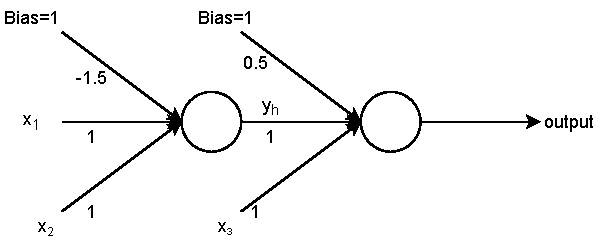
\includegraphics[scale = 0.9]{img/per2.pdf}
								\end{figure}
								con quindi una terza istanza valutata solo nel secondo livello.\\
								La funzione $f$ di attivazione del neurone è definita come quella del
								percettrone, ovvero:
								\[sgn(x)=
									\begin{cases}
										1  & \mbox{se } x\geq 0 \\
										-1 & \mbox{altrimenti}  
									\end{cases}
								\]
								L'esercizio propone di capire la label assegnata a $z_1$ e la label assegnata
								a $z_2$.\\
								Nel dettaglio, per entrambe le istanze, abbiamo $(x_1, x_2, x_3)$, ovvero i
								primi due valori sono (insieme al bias) l'input del primo layer mentre il
								terzo (insieme al bias e al risultato del primo layer) è l'input del secondo
								layer.\\
								Partiamo con $x_1=(0, 2, 2)$.\\
								Si hanno i due layer:
								\begin{enumerate}
									\item nel layer 1 si ha:
									      \[\langle \overline{x},\overline{w}\rangle=
									      	\left(\begin{matrix}
									      	1 & 0 & 2
									      	\end{matrix}\right)
									      	\left(
									      	\begin{matrix}
									      		-1.5 \\
									      		1    \\
									      		1    \\
									      	\end{matrix}
									      	\right)= -1.5+0+2 = 0.5\]
									      	Si ha quindi:
									      	\[\langle \overline{x},\overline{w}\rangle\geq 0\]
									      	e quindi:
									      	\[sgn(\langle \overline{x},\overline{w}\rangle)=sgn(0.5)=1\]
									      	avendo quindi:
									      	\[y_h=1\]
									      	che sarà tra gli input del secondo layer
									      	\item valuto quindi il layer 2:
									      	\[\langle \overline{x},\overline{w}\rangle=
									      		\left(\begin{matrix}
									      		1 & 1 & 2
									      		\end{matrix}\right)
									      		\left(
									      		\begin{matrix}
									      			-0.5 \\
									      			1    \\
									      			1    \\
									      		\end{matrix}
									      		\right)= -0.5+1+2 = 2.5\]
									      		Si ha quindi:
									      		\[\langle \overline{x},\overline{w}\rangle\geq 0\]
									      		e quindi:
									      		\[sgn(\langle \overline{x},\overline{w}\rangle)=sgn(2.5)=1\]
									      		avendo quindi:
									      		\[output=1\]
									      		\end{enumerate}
									      		Possiamo quindi dire che per la prima istanza:
									      		\[f(x_1)=+1\]
									      		Passiamo a $x_2=(1, 0, 0)$.\\
									      		Si hanno i due layer:
									      		\begin{enumerate}
									      			\item nel layer 1 si ha:
									      			      \[\langle \overline{x},\overline{w}\rangle=
									      			      	\left(\begin{matrix}
									      			      	1 & 1 & 0
									      			      	\end{matrix}\right)
									      			      	\left(
									      			      	\begin{matrix}
									      			      		-1.5 \\
									      			      		1    \\
									      			      		1    \\
									      			      	\end{matrix}
									      			      	\right)= -1.5+1+0 = -0.5\]
									      			      	Si ha quindi:
									      			      	\[\langle \overline{x},\overline{w}\rangle< 0\]
									      			      	e quindi:
									      			      	\[sgn(\langle \overline{x},\overline{w}\rangle)=sgn(-0.5)=-1\]
									      			      	avendo quindi:
									      			      	\[y_h=-1\]
									      			      	che sarà tra gli input del secondo layer
									      			      	\item valuto quindi il layer 2:
									      			      	\[\langle \overline{x},\overline{w}\rangle=
									      			      		\left(\begin{matrix}
									      			      		1 & -1 & 0
									      			      		\end{matrix}\right)
									      			      		\left(
									      			      		\begin{matrix}
									      			      			-0.5 \\
									      			      			1    \\
									      			      			1    \\
									      			      		\end{matrix}
									      			      		\right)= -0.5-1+0 = -1.5\]
									      			      		Si ha quindi:
									      			      		\[\langle \overline{x},\overline{w}\rangle < 0\]
									      			      		e quindi:
									      			      		\[sgn(\langle \overline{x},\overline{w}\rangle)=sgn(-1.5)=-1\]
									      			      		avendo quindi:
									      			      		\[output=-1\]
									      			      		\end{enumerate}
									      			      		Possiamo quindi dire che per la prima istanza:
									      			      		\[f(x_2)=-1\]
									      			      		Abbiamo quindi classificato la prima istanza come positiva e la seconda come
									      			      		negativa.
									      			      	
									      			      				\end{esercizio}
									      			      				  \section{Reti Neurali Avanzate}
							Ora che abbiamo discusso generalmente del funzionamento delle reti neurali, iniziamo a soffermarci su alcuni particolari che fanno la differenza tra un bravo e un cattivo informatico.\\ Si vuole menzionare che questi appunti sono tratti dal corso di Machine Learning, dell'università di Stanford, del professor \href{https://scholar.google.com/citations?user=mG4imMEAAAAJ&hl=it&oi=ao}{Andrew Ng}.

\subsection{Neural Networks: Representation}
							Immaginiamo di avere un layer nascosto intermedio, le cui unità vengono rappresentate dagli stati: $a_0^{(2)} \cdots a_n^{(2)}$. La seguente notazione assume questo significato:
							 \begin{itemize}
							     \item 
							$a_i^{(j)}$: attivazione dell'unità i nel layer j
							\item
							$\Theta^{(j)}$: matrice dei pesi controllanti le funzioni di mappatura dal layer j al layer j + 1.
                            	
							 \end{itemize}						
							Se abbiamo un singolo layer nascosto varrebbe la seguente formula:
							\[[ x_0 \cdots x_m ] \to [a_0^{(2)} \cdots a_n^{(2)}] \] 
							
							\textbf{NOTA: } in questa trattazione useremo $\Theta$ come $W$, essendo sinonimi in molti libri. \\
								\textbf{NOTA: } come già spiegato $x_i$ può essere visto come $a_i^{(0)}$ \\
								
							Allora possiamo riscrivere il tutto come:
							\[a_1^{(2)} = g(\Theta_{10}^{(1)}x_0 + \Theta_{11}^{(1)}x_1 + \Theta_{12}^{(1)}x_2 + \Theta_{13}^{(1)}x_3 \cdots)\] 
							\[a_2^{(2)} = g(\Theta_{20}^{(1)}x_0 + \Theta_{21}^{(1)}x_1 + \Theta_{22}^{(1)}x_2 + \Theta_{23}^{(1)}x_3 \cdots) \]
							\[a_3^{(2)} = g(\Theta_{30}^{(1)}x_0 + \Theta_{31}^{(1)}x_1 + \Theta_{32}^{(1)}x_2 + \Theta_{33}^{(1)}x_3 \cdots) \]
														\[\cdots\]

							\[h_\Theta(x) = a_1^{(3)} = g(\Theta_{10}^{(2)}a_0^{(2)} + \Theta_{11}^{(2)}a_1^{(2)} + \Theta_{12}^{(2)}a_2^{(2)} + \Theta_{13}^{(2)}a_3^{(2)} \cdots) \]

							\begin{definizione}
	Se una rete possiede $s_j$ unità nel layer $j$ e $s_{j+1}$ nel layer $j+1$, allora $\Theta^{(j)}$ avrà dimensioni pari a $s_{j+1} \times (s_j + 1)$.
	Dove $(s_j + 1)$ nasce dall'inserimento in $\Theta^{(j)}$ del nodo \textbf{bias}.
	\end{definizione}
							\begin{figure}[h!]
							\centering
							\psscalebox{0.8 0.8} % Change this value to rescale the drawing.
							{
								\begin{pspicture}(-3,-4.18)(7.52, 4.18)
									\definecolor{colour2}{rgb}{0.96862745, 0.3019608, 0.3019608}
									\definecolor{colour1}{rgb}{0.003921569, 0.003921569, 0.003921569}
									\definecolor{colour3}{rgb}{0.039215688, 0.5647059, 0.1882353}
									\definecolor{colour4}{rgb}{0.078431375, 0.28627452, 0.8784314}
									\pscircle[linecolor=black, linewidth=0.04, dimen=outer]
									(2.4, 2.7049024){0.4}
									\pscircle[linecolor=black, linewidth=0.04, dimen=outer]
									(2.4, 0.70490235){0.4}
									\pscircle[linecolor=black, linewidth=0.04, dimen=outer]
									(4.0, 0.70490235){0.4}
									\pscircle[linecolor=black, linewidth=0.04, dimen=outer]
									(0.8, 0.70490235){0.4}
									\pscircle[linecolor=black, linewidth=0.04, dimen=outer]
									(2.4,-0.8950977){0.4}
									\pscircle[linecolor=black, linewidth=0.04, dimen=outer]
									(4.0,-0.8950977){0.4}
									\pscircle[linecolor=black, linewidth=0.04, dimen=outer]
									(0.8,-0.8950977){0.4}
									\pscircle[linecolor=black, linewidth=0.04, dimen=outer]
									(1.6,-2.8950977){0.4}
									\pscircle[linecolor=black, linewidth=0.04, dimen=outer]
									(3.2,-2.8950977){0.4}
									\psline[linecolor=black, linewidth=0.04, arrowsize=0.05291667cm 2.0,
									arrowlength=1.4, arrowinset=0.0]{<-}(2.4, 2.3049023)(0.8, 1.1049024)
									\psline[linecolor=black, linewidth=0.04, arrowsize=0.05291667cm 2.0,
									arrowlength=1.4, arrowinset=0.0]{<-}(2.4, 2.3049023)(2.4, 1.1049024)
									\psline[linecolor=black, linewidth=0.04, arrowsize=0.05291667cm 2.0,
									arrowlength=1.4, arrowinset=0.0]{<-}(2.4, 2.3049023)(4.0, 1.1049024)
									\psline[linecolor=black, linewidth=0.04, arrowsize=0.05291667cm 2.0,
									arrowlength=1.4, arrowinset=0.0]{<-}(0.8,-1.2950977)(1.6,-2.4950976)
									\psline[linecolor=black, linewidth=0.04, arrowsize=0.05291667cm 2.0,
									arrowlength=1.4, arrowinset=0.0]{<-}(0.8,-1.2950977)(3.2,-2.4950976)
									\psline[linecolor=black, linewidth=0.04, arrowsize=0.05291667cm 2.0,
									arrowlength=1.4, arrowinset=0.0]{<-}(2.4,-1.2950977)(1.6,-2.4950976)
									\psline[linecolor=black, linewidth=0.04, arrowsize=0.05291667cm 2.0,
									arrowlength=1.4, arrowinset=0.0]{<-}(2.4,-1.2950977)(3.2,-2.4950976)
									\psline[linecolor=black, linewidth=0.04, arrowsize=0.05291667cm 2.0,
									arrowlength=1.4, arrowinset=0.0]{<-}(4.0,-1.2950977)(3.2,-2.4950976)
									\psline[linecolor=black, linewidth=0.04, arrowsize=0.05291667cm 2.0,
									arrowlength=1.4, arrowinset=0.0]{<-}(4.0,-1.2950977)(1.6,-2.4950976)
									\psdots[linecolor=black, dotsize=0.04](1.2,-0.09509765)
									\psdots[linecolor=black, dotsize=0.04](1.6,-0.09509765)
									\psdots[linecolor=black, dotsize=0.04](2.0,-0.09509765)
									\psdots[linecolor=black, dotsize=0.04](2.8,-0.09509765)
									\psdots[linecolor=black, dotsize=0.04](3.2,-0.09509765)
									\psdots[linecolor=black, dotsize=0.04](3.6,-0.09509765)
									\psframe[linecolor=colour2, linewidth=0.04, dimen=outer]
									(4.4,-2.0950975)(0.4,-3.6950977)
									\rput[bl](1.2,-4.0950975){\textcolor{colour1}{$a^{(j-1)}$}}
									\rput[bl](1, 3.6049025){\textcolor{colour1}{$a^{(j+1)}$}}
									\rput[bl](5,-0.19509765){\textcolor{colour1}{$a^{(j)}$}}
									\psframe[linecolor=colour3, linewidth=0.04, dimen=outer]
									(4.0, 3.5049024)(0.8, 1.9049023)
									\psframe[linecolor=colour4, linewidth=0.04, dimen=outer]
									(4.8, 1.5049024)(0.0,-1.6950977)
								\end{pspicture}
							}
						\end{figure}
	Si può definire un'implementazione vettoriali delle funzioni sopra descritte mediante la variabile $z_k^{(j)}$:
	\[a_1^{(2)} = g(z_1^{(2)})\]
\[ a_2^{(2)} = g(z_2^{(2)})\]
\[ a_3^{(2)} = g(z_3^{(2)})\]
In altre parole, per $j=2$ e un numero $k$ di nodi:
 \[z_k^{(2)} = \Theta_{k,0}^{(1)}x_0 + \cdots \Theta_{k,n}^{(1)}x_n\]
 La rappresentazione di $x$ e $z^{(j)}$ è:
 \begin{align*}x = \begin{bmatrix}x_0 \newline x_1 \newline\cdots \newline x_n\end{bmatrix} &z^{(j)} = \begin{bmatrix}z_1^{(j)} \newline z_2^{(j)} \newline\cdots \newline z_n^{(j)}\end{bmatrix}\end{align*}
 Impostando $x=a^{(1)}$ possiamo riscrivere il tutto come:
 \[z^{(j)} = \Theta^{(j-1)}a^{(j-1)}\]
 Da cui si deriva che:
 \[a^{(j)} = g(z^{(j)})\]
 \[h_\Theta(x) = a^{(j+1)} = g(z^{(j+1)})\]
\begin{esempio}
    Una semplice applicazione di una rete neurale riguarda la strutturazione di una rete per un \textbf{AND} logico. Utilizzeremo un percettrone che sfrutta una funzione logistica $g$.\\
    \textbf{NOTA:} $g(-4.6) \approx 0$ e $g(4.6) \approx 1$ 
    \begin{align}\begin{bmatrix}x_0 \nonumber \\ x_1 \nonumber \\ x_2\end{bmatrix} \rightarrow\begin{bmatrix}g(z^{(2)})\end{bmatrix} \rightarrow h_\Theta(x)\end{align}
    Inseriamo i seguenti pesi:
    \[\Theta^{(1)} = \begin{bmatrix}-30\,\,\,20\,\,\,20\end{bmatrix}\]
    Da essi avremo:
    \begin{align}& h_\Theta(x) = g(-30 + 20x_1 + 20x_2) \nonumber \\ & x_1 = 0 \ \ and \ \ x_2 = 0 \ \ then \ \ g(-30) \approx 0 \nonumber \\ & x_1 = 0 \ \ and \ \ x_2 = 1 \ \ then \ \ g(-10) \approx 0 \nonumber \\ & x_1 = 1 \ \ and \ \ x_2 = 0 \ \ then \ \ g(-10) \approx 0 \nonumber \\ & x_1 = 1 \ \ and \ \ x_2 = 1 \ \ then \ \ g(10) \approx 1 \nonumber \end{align}
    \label{AND}
\end{esempio}
L'esempio \ref{AND} si può riproporre anche per altri operatori logici: NOR oppure OR.
\begin{esempio}
    \begin{align}AND:\newline\Theta^{(1)} &=\begin{bmatrix}-30 & 20 & 20\end{bmatrix} \nonumber \\ NOR:\newline\Theta^{(1)} &= \begin{bmatrix}10 & -20 & -20\end{bmatrix} \nonumber \\ OR:\newline\Theta^{(1)} &= \begin{bmatrix}-10 & 20 & 20\end{bmatrix} \nonumber \\\end{align}
    Prese tali matrici dei pesi, possiamo combinare le corrispettive reti neurali per crearne una adatta allo \textbf{XNOR}. Per far ciò sfruttiamo le reti neurali multistrato con due layer nascosti.
    \begin{align}\begin{bmatrix}x_0 \nonumber \\ x_1 \nonumber \\ x_2\end{bmatrix} \rightarrow\begin{bmatrix}a_1^{(2)} \nonumber \\ a_2^{(2)} \end{bmatrix} \rightarrow\begin{bmatrix}a^{(3)}\end{bmatrix} \rightarrow h_\Theta(x)\end{align}
    \begin{figure}[H]
        \centering
        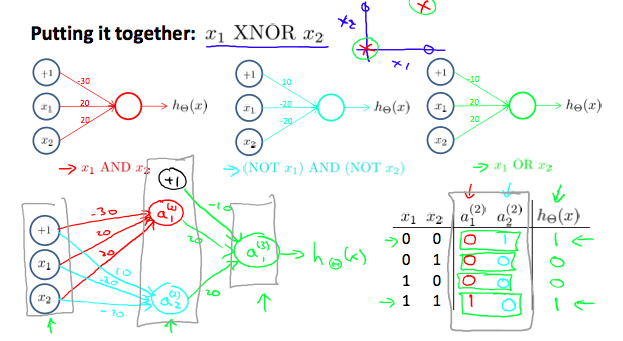
\includegraphics[width=1.0\textwidth]{img/rag_zbGqEeaSmhJaoV5QvA_52c04a987dcb692da8979a2198f3d8d7_Screenshot-2016-11-23-10.28.41.png}
        \caption{Implementazione XNOR}
        \label{XORImplementation}
    \end{figure}
\end{esempio}
\subsection{Backpropagation Algorithm}
\subsubsection{Cost function and Backpropagation}
\begin{definizione}
    Siano:
    \begin{itemize}
        \item L = numero totali di layers nella rete.
        \item $s_l$ = numero di unità (senza il bias) per il layer 'l'.
        \item K = numero di unità di output.
    \end{itemize}
    Denotando con $h_\Theta(x)_k$ l'ipotesi risultante dal $k-esimo$ ($k^{th}$) output. \\ Allora la funzione di costo per una generica rete neurale è data da:
    \small \[ J(\Theta) = - \frac{1}{m} \sum_{i=1}^m \sum_{k=1}^K \left[y^{(i)}_k \log ((h_\Theta (x^{(i)}))_k) + (1 - y^{(i)}_k)\log (1 - (h_\Theta(x^{(i)}))_k)\right] +  \frac{\alpha}{2m}\sum_{l=1}^{L-1} \sum_{i=1}^{s_l} \sum_{j=1}^{s_{l+1}} ( \Theta_{j,i}^{(l)})^2\]
\end{definizione}
Il \textbf{BackPropagation} è una terminologia inerente alle reti neurali (da non confondere con il \textbf{ForwardPropagation}) atta a minimizzare il costo della funzione $J(\Theta)$. L'obiettivo è quello di usare la \textbf{discesa del gradiente}, quindi calcolare:
\[\min_\Theta J(\Theta)\]
In particolare vogliamo minimizzare la nostra funzione di costo usando un insieme di parametri in $\Theta$. Ci occuperemo quindi di analizzare l'equazione che useremo per computare la \textbf{derivata parziale} di $J(\Theta)$:
\[\frac{\partial}{\partial \Theta_{i,j}^{(l)}} J(\Theta)\]
Per farlo sfruttiamo il \textbf{Backpropagation Algorithm}.
\begin{algorithm}[H]
	\begin{algorithmic}
		\Function{Backpropagation Algorithm}{}
		\State \textit{Training set ${(x^{(1)}, y^{(1)}) \dots (x^{(m)}, y^{(m)}) }$}
		\For {\textbf{all} (l,i,j)}
		\State {$\Delta^{(l)}_{i,j} := 0$ \textit{\color{gray}\# (hence you end up having a matrix full of zeros)}}
		\EndFor
				\State{}
		\For {\textit{Ogni esempio $t$ from $1$ to $m$}}
% 		\State {\textit{\color{gray}\# GRADIEND COMPUTATION}}
		\State Set $a^{(1)} := x^{(t)}$
		\For{l=2,3,…,L}
		\State Perform forward propagation to compute $a^{(l)}$ 
		\EndFor
% 		\State {\textit{\color{gray}\# END GRADIEND COMPUTATION}}
				\State{}
		\State {\textit{ Using $y^{(t)}$ compute $\delta^{(L)} = a^{(L)} - y^{(t)}$ \color{gray}\# \\ Where L is our total number of layers and $a^{(L)}$ is the vector of outputs of the activation units for the last layer. So our "error values" for the last layer are simply the differences of our actual results in the last layer and the correct outputs in y. To get the delta values of the layers before the last layer, we can use an equation that steps us back from right to left:}}
				\State{}
		\State {\textit{$\delta^{(l)} = ((\Theta^{(l)})^T \delta^{(l+1)})\ .*\ a^{(l)}\ .*\ (1 - a^{(l)})$ \color{gray}\# Compute $\delta^{(L-1)}, \delta^{(L-2)},\dots,\delta^{(2)}$ \\ The delta values of layer l are calculated by multiplying the delta values in the next layer with the theta matrix of layer l. We then element-wise multiply that with a function called g', or g-prime, which is the derivative of the activation function g evaluated with the input values given by $z^{(l)}$.The g-prime derivative terms can also be written out as:\\
		$g′(z^{(l)})=a^{(l)} .∗ (1−a^{(l)})$}}
		\State{}
		\State {\textit{$\Delta^{(l)}_{i,j} := \Delta^{(l)}_{i,j} + a_j^{(l)} \delta_i^{(l+1)}$ \color{gray}\# or with vectorization, $\Delta^{(l)} := \Delta^{(l)} + \delta^{(l+1)}(a^{(l)})^T$}}
				\State{}
		\State {\textit{\color{gray}\# Hence we update our new $\Delta$ matrix.\\
    $D^{(l)}_{i,j} := \dfrac{1}{m}\left(\Delta^{(l)}_{i,j} + \alpha\Theta^{(l)}_{i,j}\right)$ if $j\neq 0$\\\\
    $D^{(l)}_{i,j} := \dfrac{1}{m}\Delta^{(l)}_{i,j}$ If $j=0$ \\\\
    The capital-delta matrix D is used as an "accumulator" to add up our values as we go along and eventually compute our partial derivative. Thus we get $\frac \partial {\partial \Theta_{ij}^{(l)}} J(\Theta)=D_{ij}^{(l)}$}}
		\EndFor
		\EndFunction
	\end{algorithmic}
	\caption{Backpropagation Algorithm}
\end{algorithm}
\begin{definizione}
    Se considerassimo una semplice \textit{non-multiclass classification (k=1) } e non considerassimo la regolarizzazione ( apprendimento adattivo ) $\alpha$ avremmo un costo pari a:
    
\[cost(t) =y^{(t)} \ \log (h_\Theta (x^{(t)})) + (1 - y^{(t)})\ \log (1 - h_\Theta(x^{(t)}))\]
\end{definizione}
\begin{definizione}
    Per $\delta_j^{(l)}$ si intende l'errore per una singola unità $a^{(l)}_j$. Da cui si deriva l'uguaglianza:

\[\delta_j^{(l)} = \dfrac{\partial}{\partial z_j^{(l)}}cost(t)\]

\end{definizione}